%----------
%   IMPORTANTE
%----------

% Esta plantilla está basada en las recomendaciones de la guía "Trabajo fin de Grado: Escribir el TFG", que encontrarás en http://uc3m.libguides.com/TFG/escribir
% contiene recomendaciones de la Biblioteca basadas principalmente en estilos APA e IEEE, pero debes seguir siempre las orientaciones de tu Tutor de TFG y la normativa de TFG para tu titulación.



% ESTA PLANTILLA ESTÁ BASADA EN EL ESTILO APA


%----------
%	CONFIGURACIÓN DEL DOCUMENTO
%----------

\documentclass[12pt]{report} % fuente a 12pt

% MÁRGENES: 2,5 cm sup. e inf.; 3 cm izdo. y dcho.xx
\usepackage[
a4paper,
vmargin=2cm,
hmargin=3cm
]{geometry}

% INTERLINEADO: Estrecho (6 ptos./interlineado 1,15) o Moderado (6 ptos./interlineado 1,5)
\renewcommand{\baselinestretch}{1.25}
\parskip=12pt

% DEFINICIÓN DE COLORES para portada y listados de código
\usepackage[table]{xcolor}
\definecolor{azulUC3M}{RGB}{0,0,102}
\definecolor{gray97}{gray}{.97}
\definecolor{gray75}{gray}{.75}
\definecolor{gray45}{gray}{.45}

%colors for hightlights
\usepackage{xcolor}
\usepackage{soul}
\newcommand{\highlight}[1]{\sethlcolor{yellow}\hl{#1}}
\newcommand{\question}[1]{\sethlcolor{red}\hl{QUESTION #1}}
\newcommand{\todo}[1]{\sethlcolor{green}\hl{TODO #1}}

% Soporte para GENERAR PDF/A --es importante de cara a su inclusión en e-Archivo porque es el formato óptimo de preservación y a la generación de metadatos, tal y como se describe en http://uc3m.libguides.com/ld.php?content_id=31389625. 

% En la plantilla incluimos el archivo OUTPUT.XMPDATA. Puedes descargar este archivo e incluir los metadatos que se incorporarán al archivo PDF cuando compiles el archivo memoria.tex. Después vuelve a subirlo a tu proyecto.  
\usepackage[a-1b]{pdfx}

% ENLACES
\usepackage{hyperref}
\hypersetup{colorlinks=true,
	linkcolor=black, % enlaces a partes del documento (p.e. índice) en color negro
	urlcolor=blue} % enlaces a recursos fuera del documento en azul

% EXPRESIONES MATEMÁTICAS
\usepackage{amsmath,amssymb,amsfonts,amsthm}

% Codificación caracteres
\usepackage{txfonts} 
\usepackage[T1]{fontenc}
\usepackage[utf8]{inputenc}

\usepackage[english]{babel} 
\AtBeginEnvironment{quote}{\small}

% diseño de PIE DE PÁGINA
\usepackage{fancyhdr}
\pagestyle{fancy}
\fancyhf{}
\renewcommand{\headrulewidth}{0pt}
\rfoot{\thepage}
\fancypagestyle{plain}{\pagestyle{fancy}}

% DISEÑO DE LOS TÍTULOS de las partes del trabajo (capítulos y epígrafes o subcapítulos)
\usepackage{titlesec}
\usepackage{titletoc}
\setcounter{tocdepth}{1}
\titleformat{\chapter}[block]
{\large\bfseries\filcenter}
{\thechapter.}
{5pt}
{\MakeUppercase}
{}
\titlespacing{\chapter}{0pt}{0pt}{*3}
\titlecontents{chapter}
[0pt]                                               
{}
{\contentsmargin{0pt}\thecontentslabel.\enspace\uppercase}
{\contentsmargin{0pt}\uppercase}                        
{\titlerule*[.7pc]{.}\contentspage}                 

\titleformat{\section}
{\bfseries}
{\thesection.}
{5pt}
{}
\titlecontents{section}
[5pt]                                               
{}
{\contentsmargin{0pt}\thecontentslabel.\enspace}
{\contentsmargin{0pt}}
{\titlerule*[.7pc]{.}\contentspage}

\titleformat{\subsection}
{\normalsize\bfseries}
{\thesubsection.}
{5pt}
{}
\titlecontents{subsection}
[10pt]                                               
{}
{\contentsmargin{0pt}                          
	\thecontentslabel.\enspace}
{\contentsmargin{0pt}}                        
{\titlerule*[.7pc]{.}\contentspage}  

% DISEÑO DE TABLAS y FIGURAS
\usepackage{multirow} % permite combinar celdas 
\usepackage{caption} % para personalizar el título de tablas y figuras
\usepackage{floatrow} % utilizamos este paquete y sus macros \ttabbox y \ffigbox para alinear los nombres de tablas y figuras de acuerdo con el estilo definido.
\usepackage{array} % con este paquete podemos definir en la siguiente línea un nuevo tipo de columna para tablas: ancho personalizado y contenido centrado
\newcolumntype{P}[1]{>{\centering\arraybackslash}p{#1}}
\DeclareCaptionFormat{upper}{#1#2\uppercase{#3}\par}
\usepackage{graphicx}
\usepackage{float}
\graphicspath{{images/}} % ruta a la carpeta de imágenes

% Diseño de tabla para ciencias sociales y humanidades


% Diseño de figuras para ciencias sociales y humanidades
\captionsetup[all]{
    justification=centering,
    singlelinecheck=true,
    labelfont=bf,
    textfont=it,
    font=small,
    skip=0pt
}
\floatsetup[all]{
    heightadjust=caption,
    footposition=bottom,
    font=small
}

% Configuración del pie de las figuras y tablas 
\captionsetup*[floatfoot]{
    footfont={small, up}
}

% NOTAS A PIE DE PÁGINA
\usepackage{chngcntr} % para numeración continua de las notas al pie
\counterwithout{footnote}{chapter}

% LISTADOS DE CÓDIGO
% soporte y estilo para listados de código. Más información en https://es.wikibooks.org/wiki/Manual_de_LaTeX/Listados_de_código/Listados_con_listings
\usepackage{listings}

% definimos un estilo de listings
\lstdefinestyle{estilo}{ frame=Ltb,
	framerule=0pt,
	aboveskip=0.5cm,
	framextopmargin=3pt,
	framexbottommargin=3pt,
	framexleftmargin=0.4cm,
	framesep=0pt,
	rulesep=.4pt,
	backgroundcolor=\color{gray97},
	rulesepcolor=\color{black},
	%
	basicstyle=\ttfamily\footnotesize,
	keywordstyle=\bfseries,
	stringstyle=\ttfamily,
	showstringspaces = false,
	commentstyle=\color{gray45},     
	%
	numbers=left,
	numbersep=15pt,
	numberstyle=\tiny,
	numberfirstline = false,
	breaklines=true,
	xleftmargin=\parindent
}

\captionsetup*[lstlisting]{font=small, labelsep=period}
% fijamos el estilo a utilizar 
\lstset{style=estilo}
\renewcommand{\lstlistingname}{\uppercase{Código}}


%BIBLIOGRAFÍA 

% CONFIGURACIÓN PARA LA BIBLIOGRAFÍA APA
\usepackage[style=apa, backend=biber, natbib=true, hyperref=true, uniquelist=false, sortcites]{biblatex}
\DeclareLanguageMapping{english}{english-apa}

% Para sustituir % por y o e
\makeatletter
\DefineBibliographyExtras{english}{%
  \setcounter{smartand}{1}%
  \let\lbx@finalnamedelim=\lbx@en@smartand
  \let\lbx@finallistdelim=\lbx@en@smartand
}

\makeatother


\addbibresource{referencias.bib} % llama al archivo referencias.bib en el que deberá estar la bibliografía utilizada


%-------------
%	DOCUMENTO
%-------------

% Dont split paragraphs between page breaks
\widowpenalties 1 10000
\raggedbottom

% make sections in a new page
\let\oldsection\section
\renewcommand\section{\clearpage\oldsection}
\usepackage{etoolbox}
\usepackage{titlesec}
\usepackage{lipsum} % for dummy text, you can remove this in your actual document

\titleformat{\chapter}[display]
  {\normalfont\huge\bfseries\centering}{\chaptertitlename\ \thechapter}{20pt}{\Huge}

\titleformat{\section}
  {\normalfont\Large\bfseries\centering}{\thesection}{1em}{}

\makeatletter
\pretocmd{\chapter}{\if@openright\cleardoublepage\else\clearpage\fi\thispagestyle{empty}}{}{}
\makeatother

\begin{document}
\pagenumbering{roman} % Se utilizan cifras romanas en la numeración de las páginas previas al cuerpo del trabajo
	
%----------
%	PORTADA
%----------	
\begin{titlepage}
	\begin{sffamily}
	\color{azulUC3M}
	\begin{center}
		\begin{figure}[H] %incluimos el logotipo de la Universidad
			\makebox[\textwidth][c]{
\includegraphics[width=16cm]{logo_UC3M.png}}
		\end{figure}
		\vspace{2.5cm}
		\begin{Large}
			\vspace{2cm}		
			\textsl{High Frequency Technology}
			\bigskip
			
		\end{Large}
		 	{\Huge Design of a two-stage, balanced amplifier}\\
		 	\vspace*{0.5cm}
	 		\rule{10.5cm}{0.1mm}\\
			\vspace*{0.9cm}
			{\LARGE Andrés Navarro Pedregal (100451730)}\\ 
            {\LARGE \&}\\
			{\LARGE Daniel Toribio Bruna (100454242)}\\ 
			\vspace*{1cm}
	\vfill
		\begin{Large}
			\today
		\end{Large}
	\end{center}
	\end{sffamily}
\end{titlepage}

\newpage %página en blanco o de cortesía
\thispagestyle{empty}
\mbox{}

%----------
%	ÍNDICES
%----------	

%--
% Índice general
%-
\tableofcontents
\thispagestyle{fancy}

\newpage % página en blanco o de cortesía
\thispagestyle{empty}


%----------
%	MEMORIA
%----------	
\clearpage
\pagenumbering{arabic} % numeración con números arábigos para el resto de la memoria.	

%--
% Report
%-------------------------------------
\chapter{Introduction}

In this laboratory exercise, we focus on designing and understanding a two-stage microwave amplifier. Our goal is to create a device that can increase the power of microwave signals efficiently for a specific frequency range. We will be using a commercial integrated amplifier called GVA-83+ for the main part of our design. We will be using microstrip technology, which is common in microwave circuits, to build our amplifier.

Amplifiers have limits, like how much power they can give out and how much they can boost the signal. To overcome these limits, we're using a two-stage design. This means we connect two amplifiers together to get more power. We're also using special techniques like splitting the signal into two parts and amplifying each part separately. Then, we combine them again to get even more power and reduce the noise induced by the amplification. This is called a balanced amplifier. Our design also includes a band pass filter to make sure we only amplify the frequency range we want. 

\section{Initial parameters}

For our case the initial parameters that we will be using will be the ones given in the Figure \ref{fig:introduction:initial_parameters}.

\begin{figure}[htbp]
    \centering
    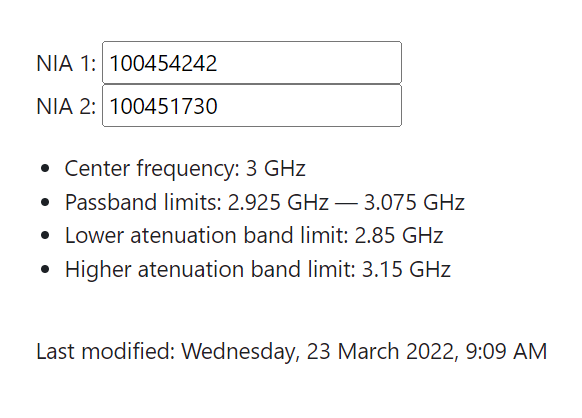
\includegraphics[width=0.65\textwidth]{introduction/initial_parameters_calculator.png}
    \caption{Initial parameters for our case study.}
    \label{fig:introduction:initial_parameters}
\end{figure}

%-------------------------------------
\chapter{Previous Work}
\section{Substrate Selection}

For the circuit design we will be using a substrate with a microstrip structure with two possible dielectric thickness of $h = 0.508 mm$ or $h = 1.27 mm$ and a thick copper metallization of $t = 17 \mu m$. For the substrate type the different configuration are seen in the Table \ref{tab:previous_work:substrate_types}.

\begin{table}[htbp]
    \centering
    \caption{Substrate types}
    \label{tab:previous_work:substrate_types}
    \begin{tabular}{@{}llll@{}}
    Material & Relative permittivity ($\varepsilon_r$) & Loss tangent ($\tan \delta$) & Cost per area \\
    Fiberglass (FR4) & 4.7 & 0.01 & $\times 1$ \\
    RT/Duroid 5880 & 2.2 & 0.009 & $\times 10$ \\
    RT/Duroid 6006 & 6.15 & 0.0027 & $\times 10$ \\
    RT/Duroid 6010.2LM & 10.2 & 0.0023 & $\times 10$ \\
    \end{tabular}
\end{table}

\subsection{Substrate type}

As we can see in table \ref{tab:previous_work:substrate_types}, the \textit{Fiberglass (FR4)} has a really high loss tangent $\tan \delta$. Even though it is the cheapest, we have decided to use another substrate that has a better $\tan \delta$ in order to improve our amplifier. For the choices, we can only choose the \textit{RT/Duroid 6006} or the \textit{RT/Duroid 6010.2LM} as the \textit{RT/Duroid 5880} as almost the same $\tan \delta$ as \textit{Fiberglass (FR4)}.

Comparing the  \textit{RT/Duroid 6006} and the \textit{RT/Duroid 6010.2LM}, we can observe that they have the same price so we will go with the one with the lowest $\tan \delta$. That is as we want to reduce the losses at maximum. So let's study the \textit{RT/Duroid 6010.2LM}. 

If we use the values given the in the Table \ref{tab:previous_work:substrate_types} for the \textit{RT/Duroid 6010.2LM} and the AWR TXLine tool, we get a microstrip width of $w = 0.458 $ when the dielectric thickness of $h = 0.508 mm $ for a $Z = 50 \Omega$ (See Figure \ref{fig:previous_work:duroid_6010.2lm_h_1_27_mm_50_ohm}). On the other hand, if we use a $h = 1.27 mm$ for a $Z = 50 \Omega$, we get a microstrip width of $w = 1.17 mm$ which is larger (See Figure \ref{fig:previous_work:duroid_6010.2lm_h_1_27_mm_50_ohm}.

\begin{figure}[htbp]
    \centering
    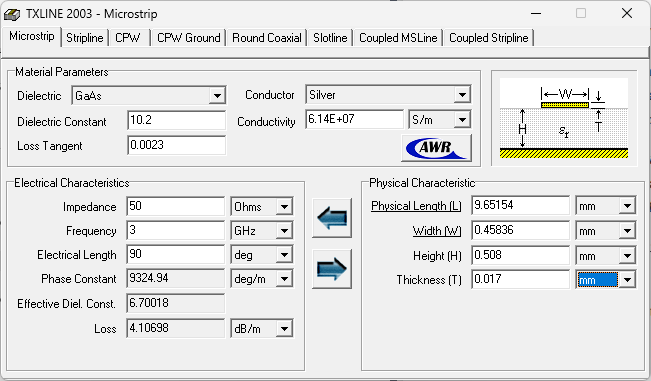
\includegraphics[width=\textwidth]{images/previous_work/txline_tool_duroid_6010.2lm_h_0_508_mm_50_ohm.png}
    \caption{Width $w = 0.458 mm$ for RT/Duroid 6010.2LM with $h = 0.508 mm$ and a $Z = 50 \Omega$}
    \label{fig:previous_work:duroid_6010.2lm_h_0_508_mm_50_ohm}
\end{figure}

\begin{figure}[htbp]
    \centering
    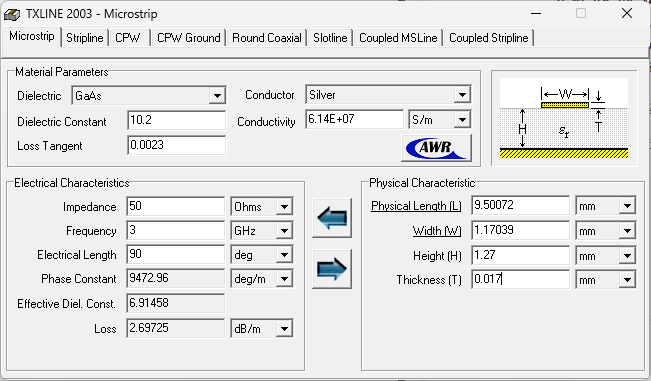
\includegraphics[width=\textwidth]{images/previous_work/txline_tool_duroid_6010.2lm_h_1_27_mm_50_ohm.png}
    \caption{Width $w = 1.17 mm$ for RT/Duroid 6010.2LM with $h = 1.27 mm$ and a $Z = 50 \Omega$}
    \label{fig:previous_work:duroid_6010.2lm_h_1_27_mm_50_ohm}
\end{figure}

Considering that the width of each line must be no less than $200 \mu m$, both lines would work perfectly fine at $Z = 50 \Omega$. However, as we are designing a circuit where we might need different values of $Z$, we will see if they still work for for example $Z = 100 \Omega$.

Using the \textit{RT/Duroid 6010.2LM} with  a dielectric thickness of $h = 1.27 mm$ for $Z = 100 \Omega$ we get a microstrip width of $w = 0.144mm$ (See Figure \ref{fig:previous_work:duroid_6010.2lm_h_1_27_mm_100_ohm}). As the width needed, is smaller than the one required, this substrate it is not the most recommended.

\begin{figure}[htbp]
    \centering
    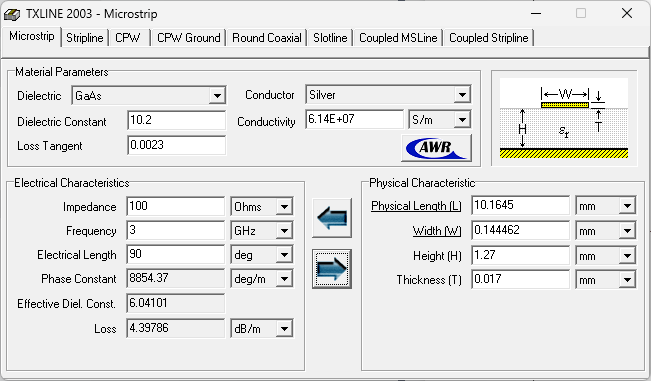
\includegraphics[width=\textwidth]{images/previous_work/txline_tool_duroid_6010.2lm_h_1_27_mm_100_ohm.png}
    \caption{Width $w = 0.144 mm$ for RT/Duroid 6010.2LM with $h = 1.27 mm$ and a $Z = 100 \Omega$}
    \label{fig:previous_work:duroid_6010.2lm_h_1_27_mm_100_ohm}
\end{figure}

Due to that inconvenience, let's study the substrate \textit{RT/Duroid 6006}. For this substrate with a $h = 1.27 mm$ and a $Z = 100 \Omega$, we get a width of $w = 0.343 mm$ (See Figure \ref{fig:previous_work:duroid_6006_h_1_27_mm_100_ohm}). This width is much better than the \textit{RT/Duroid 6010.2LM} with the $200 \mu m$ minimum width constraint as we have more room to design our circuit. Therefore, we will be using the \textit{RT/Duroid 6006}.

\begin{figure}[htbp]
    \centering
    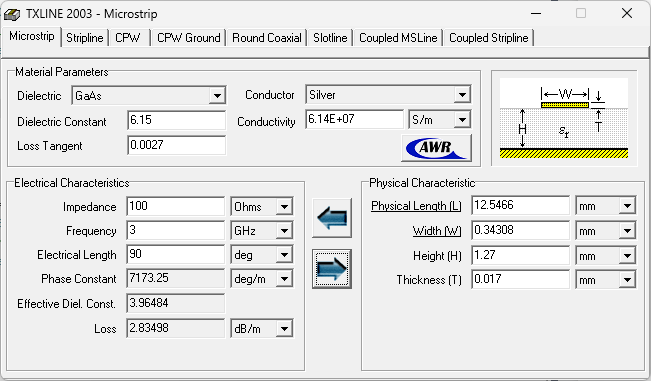
\includegraphics[width=\textwidth]{images/previous_work/txline_tool_duroid_6006_h_1_27_mm_100_ohm.png}
    \caption{Width $w = 0.343 mm$ for RT/Duroid 6006 with $h = 1.27 mm$ and a $Z = 100 \Omega$}
    \label{fig:previous_work:duroid_6006_h_1_27_mm_100_ohm}
\end{figure}

\subsection{Substrate dielectric thickness}

For the dielectric thickness, we can see in Figure \ref{fig:previous_work:duroid_6006_h_0_508_mm_100_ohm} that for the \textit{RT/Duroid 6006} with a $h = 0.508 mm$ and a $Z = 100 \Omega$, we get a width of $w = 0.128$. As stated before, that does not check the constraint of a minimum width of $w = 0.2 mm$. Because of that we will select a dielectric thickness of $h = 1.27 mm$.

\begin{figure}[htbp]
    \centering
    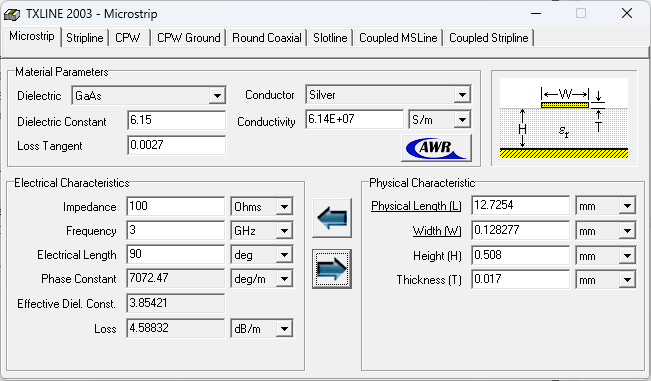
\includegraphics[width=\textwidth]{images/previous_work/txline_tool_duroid_6006_h_0_508_mm_100_ohm.png}
    \caption{Width $w = 0.128 mm$ for RT/Duroid 6006 with $h = 0.508 mm$ and a $Z = 100 \Omega$}
    \label{fig:previous_work:duroid_6006_h_0_508_mm_100_ohm}
\end{figure}

\subsection{Final substrate selection}

For the substrate, we will select the \textit{RT/Duroid 6006} as it is the best one for the same price that fits the constraints required. For the dielectric thickness, we will use a $h = 1.27 mm$ for the very same reason. Choosing this dielectric will make our circuit as small as possible while keeping the losses at minimum. The price is not a concern as the \textit{Fiberglass (FR4)}, even though it is the cheapest, we decided to discarded due to its really high $\tan \delta$. And among the rest of the substrates, the price is the same.

Finally, in the Figure \ref{fig:previous_work:duroid_6006_h_1_27_mm_50_ohm}, we can see the calculations of the final width of $w = 1.85 mm$ for a characteristic impedance of $Z_{0} = 50 \Omega$ and a dielectric thickness of $h = 1.27 mm$. As we can see, the width is bigger than $w = 200 \mu m$, therefore it checks the constraints and it will be the one we will be using further on.

\begin{figure}[htbp]
    \centering
    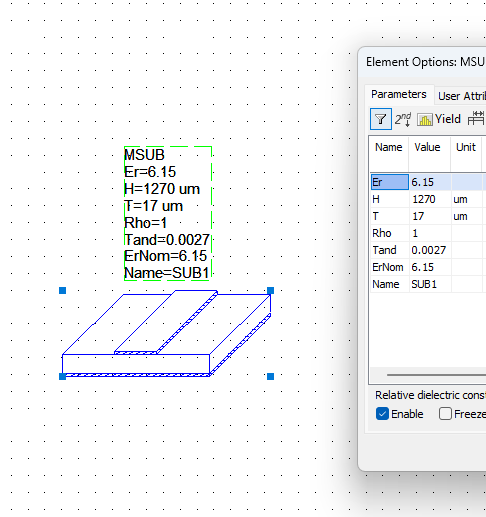
\includegraphics[width=0.75\textwidth]{images/previous_work/final_substrate_duroid_6006_h_1_27_mm.png}
    \caption{Final substrate selection}
    \label{fig:previous_work:final_substrate}
\end{figure}

\begin{figure}[htbp]
    \centering
    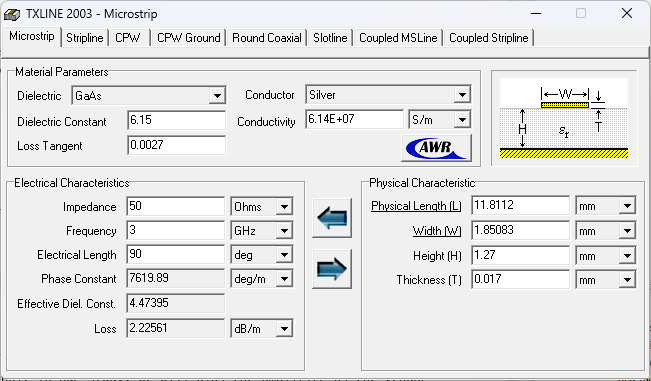
\includegraphics[width=\textwidth]{images/previous_work/txline_tool_duroid_6006_h_1_27_mm_50_ohm.png}
    \caption{Width $w = 1.85 mm$ for RT/Duroid 6006 with $h = 1.27 mm$ and a $Z = 50 \Omega$}
    \label{fig:previous_work:duroid_6006_h_1_27_mm_50_ohm}
\end{figure}

\chapter{Design of the Circuit Elements}
\section{First Stage: Simple Amplifier}

For the amplifier, we will be using the GVA83+, which is a wide band amplifier for a dynamic range of applications. In order for an amplifier to work, it needs to be supplied a DC power in order for it to perform the amplification of our signal. In our study, we will bias the amplifier as the vendor recommends, see Figure \ref{fig:design_circuit_elements:gva83+_bias_configuration}. 

\begin{figure}[htbp]
    \centering
    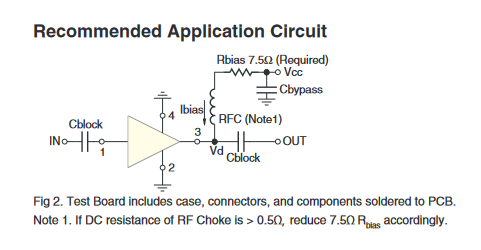
\includegraphics[width=\textwidth]{images/design_circuit_elements/gva83+_bias_configuration.png}
    \caption{Bias network of the GVa83+ Amplifier recommended by the vendor}
    \label{fig:design_circuit_elements:gva83+_bias_configuration}
\end{figure}

\subsection{Analysis of the Bias Network (Figure \ref{fig:design_circuit_elements:gva83+_bias_configuration}) at f = 0 GHz and f = 3 GHz}

When $f = 0 GHz$, we can observe that the impedance of the capacitors $Z_{C} = \frac{1}{j \cdot 2 \cdot \pi \cdot f \cdot C} \xrightarrow{} \infty$ when $f \xrightarrow{} 0$ acting as an open circuit. On the other hand, the impedance of the inductor $Z_{L} = j \cdot 2 \cdot \pi \cdot f \cdot L \xrightarrow{} 0$ when $f \xrightarrow{} 0$ acting as a short circuit. Taking those points into account, we get that the circuit can be summarized as seen in Figure \ref{fig:design_circuit_elements:gva83+_bias_f_0_ghz} when $f = 0 GHz$. Since the output is not connected to the input, then the circuit will not work at very low frequencies. However, we can calculate the current flowing through the inductor as it is a short circuit now, and that current will be the one in charge of powering the amplifier. In this case $I_{bias} = \frac{V_{CC}}{R_{bias}}$ .

\begin{figure}[htbp]
    \centering
    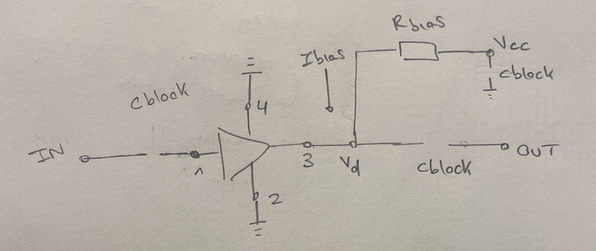
\includegraphics[width=\textwidth]{images/design_circuit_elements/gva83+_bias_f_0_ghz.png}
    \caption{Bias network of the GVa83+ Amplifier at $f = 0 GHz$}
    \label{fig:design_circuit_elements:gva83+_bias_f_0_ghz}
\end{figure}

On the other hand, if we study the circuit at the designed frequency $f = 3 GHz$; the capacitors act as a short circuit and the inductor act as an open circuit. That way, the branch required to bias the amplifier is "disconnected" per say (See Figure \ref{fig:design_circuit_elements:gva83+_bias_f_3_ghz}) and the gain of the amplifier is $G = Av = s_{21}$.

\begin{figure}[htbp]
    \centering
    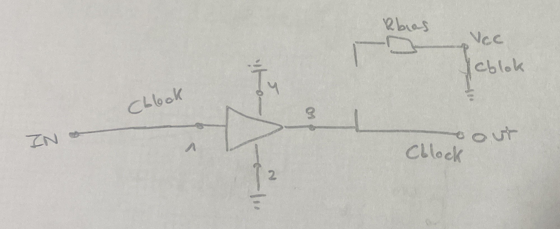
\includegraphics[width=\textwidth]{images/design_circuit_elements/gva83+_bias_f_3_ghz.png}
    \caption{Bias network of the GVA83+ Amplifier at $f = 3 GHz$}
    \label{fig:design_circuit_elements:gva83+_bias_f_3_ghz}
\end{figure}

\subsection{Analysis of the Bias Network (Figure \ref{fig:design_circuit_elements:gva83+_bias_configuration}) with the Transmission Line at f = 0 GHz and f = 3 GHz}

The analysis of the proposed Bias Network with the Transmission Line (TL) (see Figure \ref{fig:design_circuit_elements:gva83+_bias_transmission_line}) is really similar to the one proposed by the vendor (see Figure \ref{fig:design_circuit_elements:gva83+_bias_configuration}). The only differences are that we are using a TL instead of an inductor and the bypass capacitor now it is in parallel with the TL.

At $f = 0 GHz$, the capacitors act as open circuits and the TL acts as a short circuit. Again, since the output is not connected to the amplifier, the circuit does not work as previously stated. On the other hand, at $f = 3 GHz$, the capacitors act as a short circuit and the TL acts as an open circuit as before. The gain of the circuit is still the same as before $G = Av = s{21}$.

Now if we study the inductor, we want that the inductor acts as a short circuit at $f = 0 GHz$ and as an open circuit at $f = 3 GHz$. For this, when $f = 0 GHz$, the TL acts like a normal cable so it can be neglected. Thus, the amplifier is connected to $V_{cc}$, powering up the amplifier. On the other hand, we want that at $f = 3 GHz$ the TL to act like a short circuit. We can see that as the capacitor acts like a short circuit in $f = 3 GHz$, we will have an impedance of 0 at the end of the TL between the capacitor and the resistor. So if we make the length of the TL of $l = \frac{\lambda}{4}$, we will have at the output port an impedance of $\infty$.


In order to calculate the length of the TL in order to function as the inductor, we need to get the highest possible value of the characteristic impedance ($Z_0$). For this we have used the AWR TXLine tool and we got a length of $l = 12.692 mm$ with a characteristic impedance of $Z_0 = 130.62 \Omega$ (see Figure \ref{fig:design_circuit_elements:txline_tool_bias_network_amplifier_transmission_line}). Keep in mind that we have used the minimum width available $w = 200 \mu m$ in order to make it as small as possible. The reasoning for getting the maximum $Z_0$ is because that way, the TL will behave like an open circuit for high frequencies and like a short circuit for low frequencies.

\begin{figure}[htbp]
    \centering
    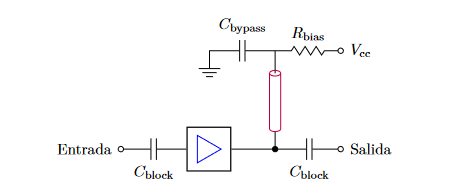
\includegraphics[width=\textwidth]{images/design_circuit_elements/gva83+_bias_transmission_line.png}
    \caption{Proposed Bias Network of the GVA83+ Amplifier with a TL}
    \label{fig:design_circuit_elements:gva83+_bias_transmission_line}
\end{figure}

\subsection{Wide band Simulation of the Vendor's Bias Network}

For the Vendor's Bias Network, we will be using the circuit pictured in Figure \ref{fig:design_circuit_elements:bias_network_vendor_circuit}. As we can see in Figure \ref{fig:design_circuit_elements:bias_network_vendor_graph}, the amplifier works as expected. It is powered by the bias network as stated before, and works correctly at our desired frequency of $f = 3 GHz$.

\begin{figure}[htbp]
    \centering
    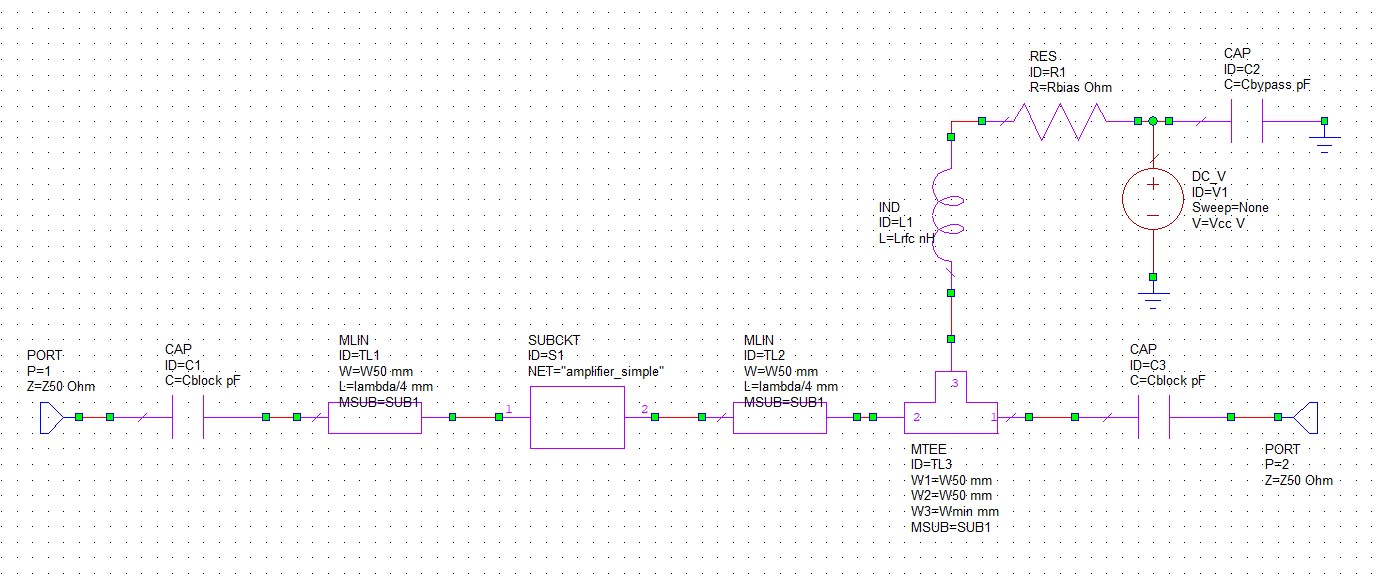
\includegraphics[width=1\linewidth]{images//design_circuit_elements/bias_network_vendor_circuit.png}
    \caption{Circuit of the vendor's bias network}
    \label{fig:design_circuit_elements:bias_network_vendor_circuit}
\end{figure}

\begin{figure}[htbp]
    \centering
    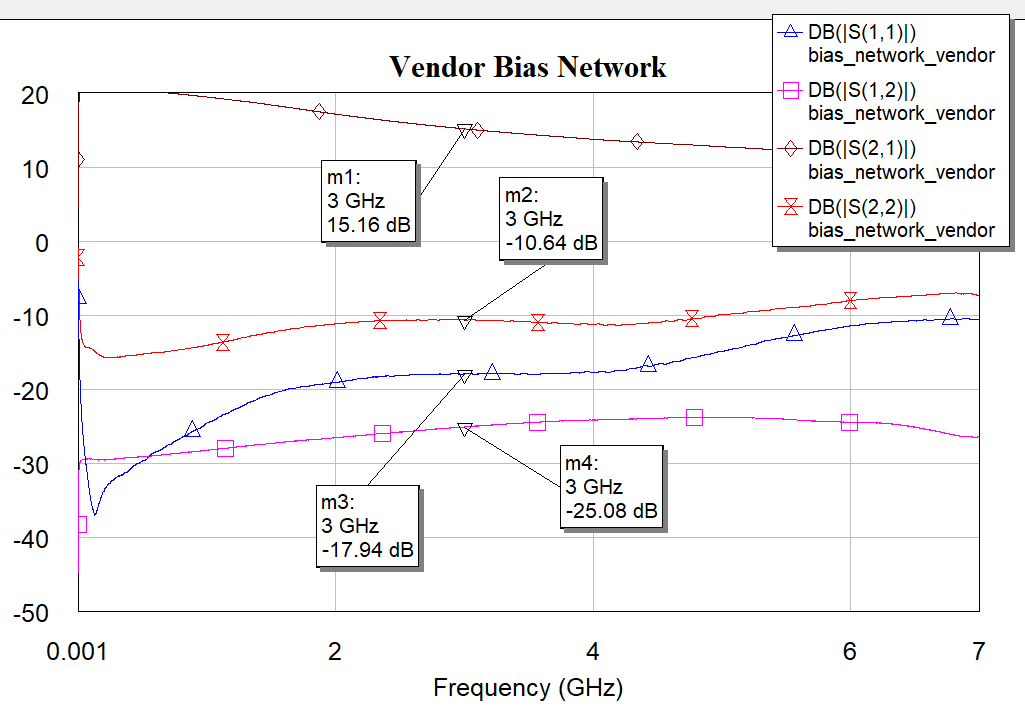
\includegraphics[width=1\linewidth]{images//design_circuit_elements/bias_network_vendor_graph.png}
    \caption{Simulation of the vendor's bias network of Figure \ref{fig:design_circuit_elements:bias_network_vendor_circuit}}
    \label{fig:design_circuit_elements:bias_network_vendor_graph}
\end{figure}

\subsection{Wide band Simulation of the Proposed Bias Network}

For the proposed bias network, we will be using the circuit shown in Figure \ref{fig:design_circuit_elements:bias_network_proposed_circuit}. And for this circuit, we get the following simulation (see Figure \ref{fig:design_circuit_elements:bias_network_proposed_graph}). If we compare it to the bias network that the vendor recommended (see Figure \ref{fig:design_circuit_elements:bias_network_vendor_graph}), we can see that the values for the S-parameters are almost the same. However, that is only for our working frequency of $f_0 = 3 GHz$. If we look at the $s_{21}$ parameter, we can see that it is smoother in the proposed network. That is because as we have the capacitor in parallel with the resistor, then the node between them will have a stable ground when working at high frequencies.

\begin{figure}[htbp]
    \centering
    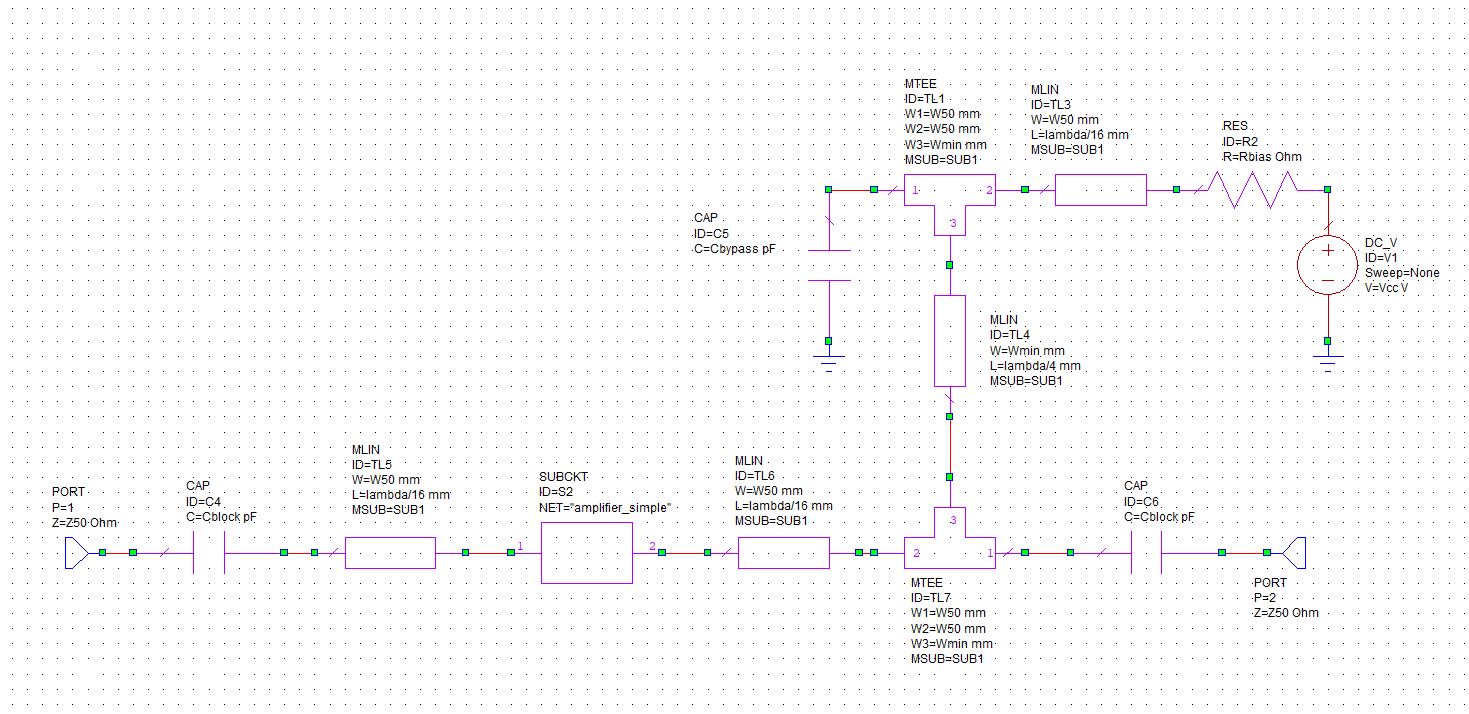
\includegraphics[width=1\linewidth]{images//design_circuit_elements/bias_network_proposed_circuit.png}
    \caption{Circuit of the proposed bias network}
    \label{fig:design_circuit_elements:bias_network_proposed_circuit}
\end{figure}

\begin{figure}[htbp]
    \centering
    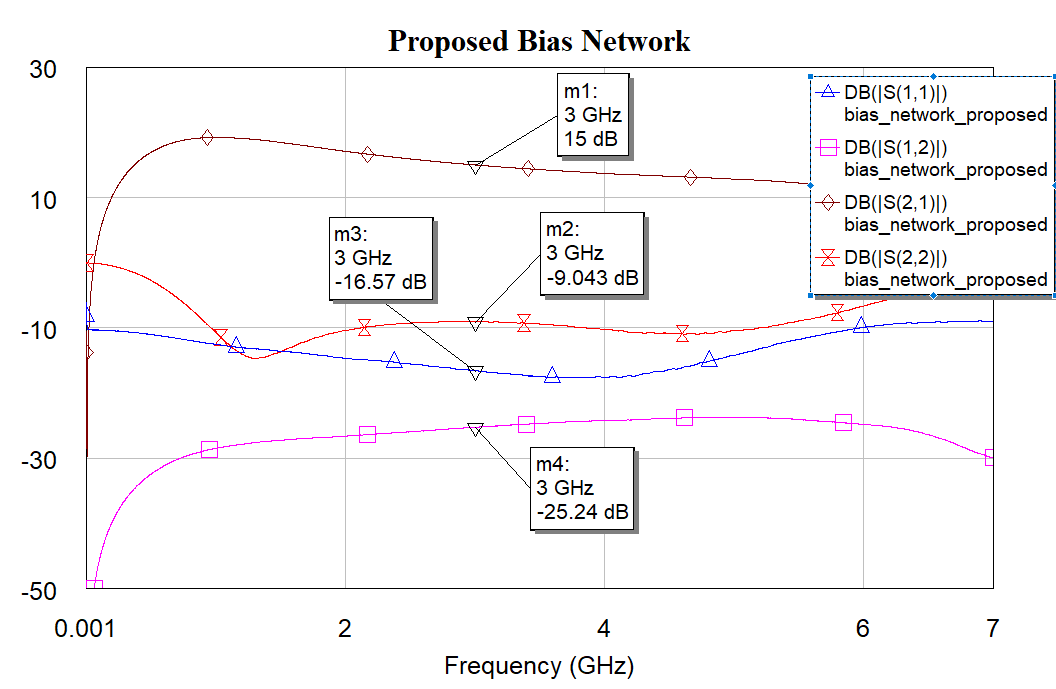
\includegraphics[width=1\linewidth]{images//design_circuit_elements/bias_network_proposed_graph.png}
    \caption{Simulation of the proposed bias network of Figure \ref{fig:design_circuit_elements:bias_network_proposed_circuit}}
    \label{fig:design_circuit_elements:bias_network_proposed_graph}
\end{figure}

If we modify the characteristic impedance of the transmission line (we will make it the same as $Z_0$), we can see in Figure \ref{fig:design_circuit_elements:gva83+_bias_transmission_line_low_z_0}, that the circuit behaves the same for the desired frequency of $f_0 = 3 GHz$. However, outside that frequency the amplification diminishes and it is not as effective as the network with the highest $Z_0$, smallest width of $w = 0.2 mm$ (see Figure \ref{fig:design_circuit_elements:bias_network_proposed_graph}). Therefore, having a really high $Z_0$ in the transmission lines assures us that the bias network will work at a wider range of frequencies than our $f_0$.

\begin{figure}[htbp]
    \centering
    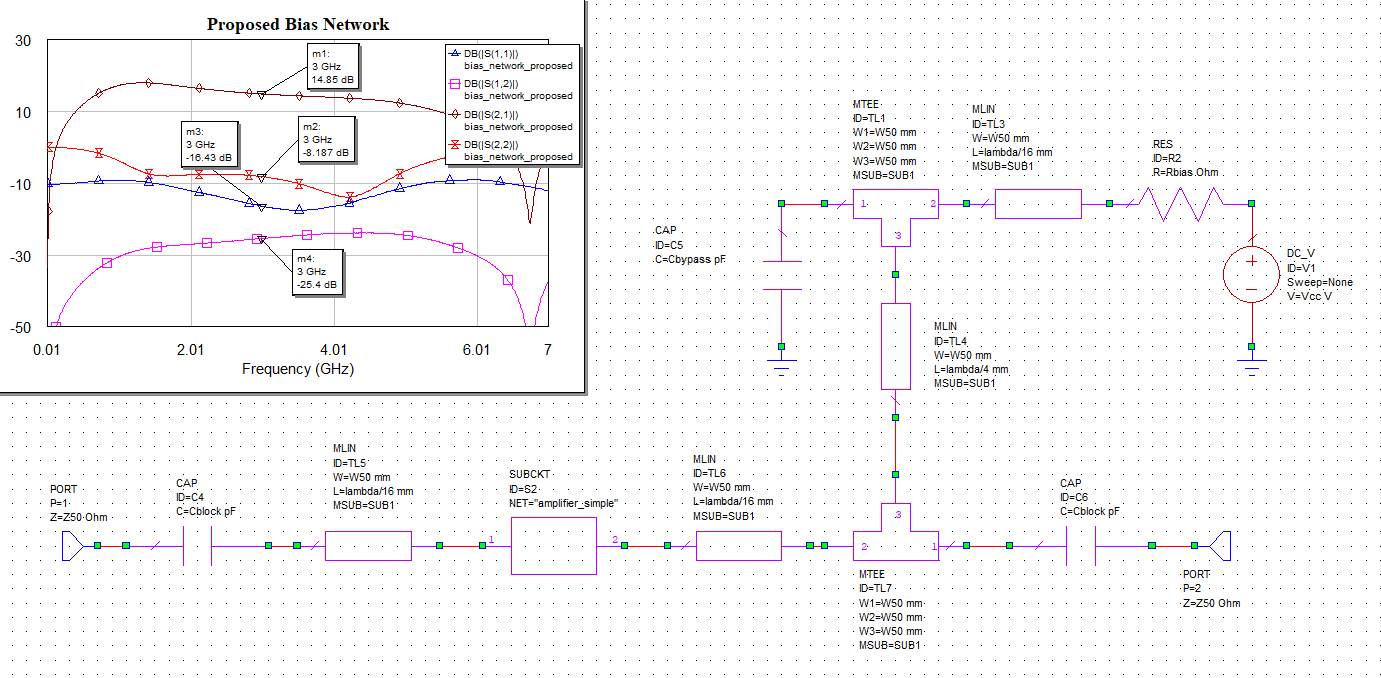
\includegraphics[width=1\linewidth]{images//design_circuit_elements/gva83+_bias_transmission_line_low_z_0.png}
    \caption{Proposed bias network with a TL width of $w = 1.85083 mm$}
    \label{fig:design_circuit_elements:gva83+_bias_transmission_line_low_z_0}
\end{figure}

\section{GVA83+ response}
 
\subsection{Scattering parameters at f = 3 GHz}

In our case, with a working frequency of f = 3 GHz (see Figure \ref{fig:introduction:initial_parameters}) and for the nominal temparture and bias conditions ($V_{CC} = 5V, R_{bias} = 7.5 \Omega$), we get the following scattering parameters:

\[
[S] = \begin{bmatrix}
s_{11} = -16.87 \ dB & \quad s_{12} = -25.06 \ dB \\
s_{21} = 15.34 \ dB & \quad s_{22} = -10.68 \ dB \\
\end{bmatrix}
\]

Where:
\begin{align*}
s_{11} & : \text{Input Return Loss} \\
s_{12} & : \text{Isolation} \\
s_{21} & : \text{Gain} \\
s_{22} & : \text{Output Return Loss}
\end{align*}

Note: this parameters are for the frequency $f = 2.9 GHz$ (see Figure \ref{fig:design_circuit_elements:scattering_parameters_datasheet}). However, that frequency is really close to our working frequency of $f = 3 GHz$ so there will be almost the same.

\begin{figure}[htbp]
    \centering
    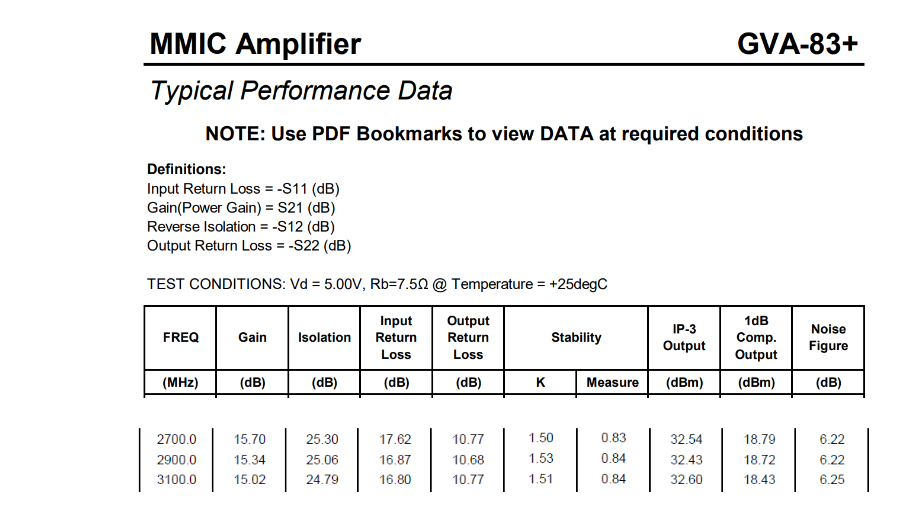
\includegraphics[width=\textwidth]{images/design_circuit_elements/scattering_parameters_datasheet.png}
    \caption{Scattering Parameters from the GVA-83+ datasheet}
    \label{fig:design_circuit_elements:scattering_parameters_datasheet}
\end{figure}

\subsection{Gain of each amplifier stage and the full two-stage network}
\label{subsec:gain_each_amplifier_and_full_two_stage}

The gain of just one amplifier is the scattering parameter $s_{21}$, so in our case the gain is $G = S{21} = 15.34 \ dB$. As the first stage and the second stage have just one amplifier, the gain of both of the will be the same of $G = 15.34 \ dB$. That is because the second stage behaves like a isolated amplifier with respect to the first stage.

For the full network, the gain of the whole circuit will be the product of both amplifiers as they are isolated to each other. That is the total gain will be $G_T = s_{21}^2$, so in dB it is $G_T = 2 \cdot s_{21} (in \ dB) = 2 * 15.34 = 30.60 \ dB$.

\subsection{Comparison of the wide band S parameters with the data sheet}

In the Figure \ref{fig:design_circuit_elements:graph_amplifier}, we can see the scattering parameters at our working frequency $f = 3 GHz$. If we take a look at each parameter, we can clearly see that they are almost the same values as the ones we obtained from the datasheet (see Figure \ref{fig:design_circuit_elements:scattering_parameters_datasheet}).

\begin{figure}[htbp]
    \centering
    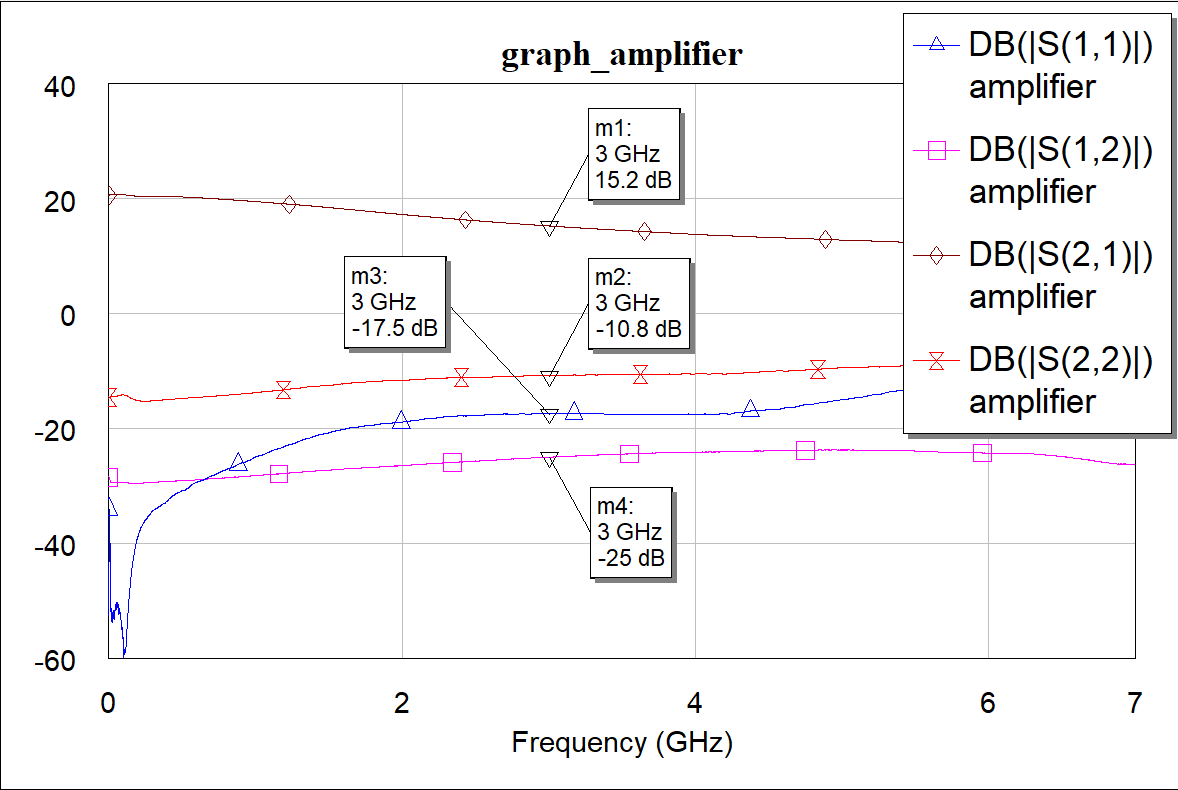
\includegraphics[width=\textwidth]{images/design_circuit_elements/graph_amplifier.png}
    \caption{AWR Graph of the GVA83+ Amplifier}
    \label{fig:design_circuit_elements:graph_amplifier}
\end{figure}

\section{Second Stage: Balanced Amplifier}

The second amplifier will be a balanced amplifier, that is a amplifier that first divides the signal into 2 signals and amplifies them separately. The idea with this amplifier, is to apply a phase shift to the signals of 180 degrees and them join them again at the end. With this configuration, as we are adding to signals that where shifted 180 degrees, any noise that we get in the amplifiers will be cancelled out resulting in a much cleaner signal.

For our case, we will have 3 different configurations depending on the order of the amplification and the phase shift. The configurations are described in Figure \ref{fig:design_circuit_elements:configurations_balanced_stage}. So let's get started and start by studying the different configurations.

Note: that for all of the configurations we will consider ideal Wilkinson combiners / dividers and a reference impedance of $Z_0 = 50 \Omega$. And we will be using the following scattering parameters:

For the Wilkinson we will be using: 

\[
[S_W] = \frac{-j}{\sqrt{2}} \* \begin{bmatrix}
0 & \quad 1 & \quad 1 \\
1 & \quad 0 & \quad 0 \\
1 & \quad 0 & \quad 0 \\
\end{bmatrix}
\]

For the amplifier:

\[
[S_A] = \begin{bmatrix}
s_{11A} & \quad s_{12A} \\
s_{21A} & \quad s_{22A} \\
\end{bmatrix}
\]

And finally for the phase shifter:

\[
[S_{\phi}] = \begin{bmatrix}
0 & \quad e^{-j \* \phi} \\
e^{-j \* \phi} & \quad 0 \\
\end{bmatrix}
\]

\begin{figure}[htbp]
    \centering
    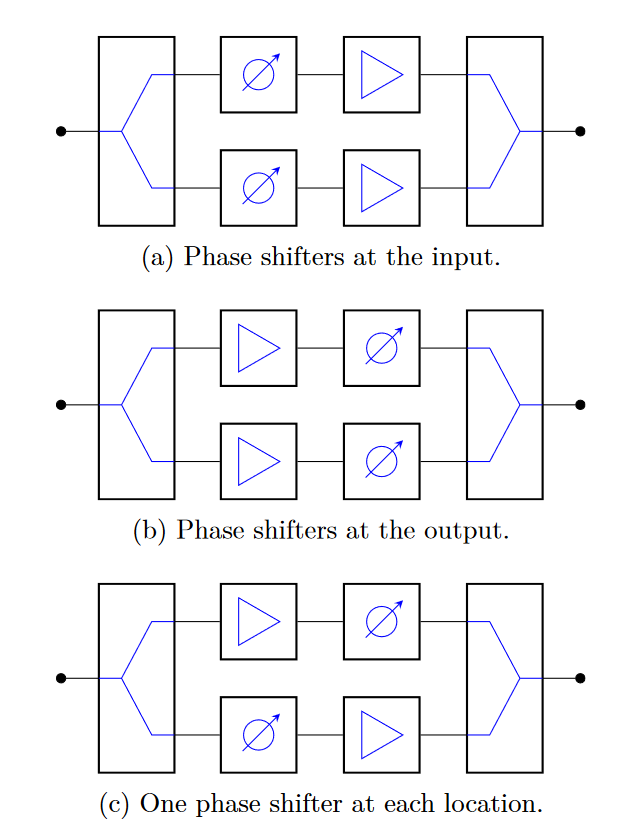
\includegraphics[width=\textwidth]{images/design_circuit_elements/configurations_balanced_stage.png}
    \caption{3 different configurations for the Balanced Stage}
    \label{fig:design_circuit_elements:configurations_balanced_stage}
\end{figure}

\subsection{S matrix for configuration (a) of Figure \ref{fig:design_circuit_elements:configurations_balanced_stage}}

For the first configuration, we get the following scattering parameters:

\[
[S] = \begin{bmatrix}
- s_{11A} \* e^{-2 \* j \* \phi} & \quad - s_{21A} \* e^{- j \* \phi} \\
- s_{21A} \* e^{- j \* \phi} & \quad - s_{22A} \\
\end{bmatrix}
\]

Note: that $s_{21} = s_{12}$ as the S matrix is reciprocal.

\subsection{S matrix for configuration (b) of Figure \ref{fig:design_circuit_elements:configurations_balanced_stage}}

For the second configuration, we get the following scattering parameters:

\[
[S] = \begin{bmatrix}
- s_{11A} & \quad - s_{21A} \* e^{- j \* \phi} \\
- s_{21A} \* e^{- j \* \phi} & \quad - s_{22A} \* e^{-2 \* j \* \phi} \\
\end{bmatrix}
\]

Note: that $s_{21} = s_{12}$ as the S matrix is reciprocal.

\subsection{S matrix for configuration (c) of Figure \ref{fig:design_circuit_elements:configurations_balanced_stage}}

Finally, for the last configuration, we get the following scattering parameters:

\[
[S] = \begin{bmatrix}
- \frac{s_{11A}}{2} \* (1 + e^{-2 \* j \* \phi}) & \quad - s_{21A} \* e^{- j \* \phi} \\
- s_{21A} \* e^{- j \* \phi} & \quad - \frac{s_{22A}}{2} \* (1 + e^{-2 \* j \* \phi}) \\
\end{bmatrix}
\]

Note: that $s_{21} = s_{12}$ as the S matrix is reciprocal.

\subsection{Comparison between the different configuration of Figure \ref{fig:design_circuit_elements:configurations_balanced_stage} and the simple amplifier}

Now that we have the 3 different S matrices, we can observe that they have the same transmission coefficients $s_{21} = s_{12} = - s_{21A} \* e^{- j \* \phi}$. That means that they will transmit the same power to the load. This makes sense as the only thing that differs between the configurations is the order of the components, but they are still the same.

On the other hand, if we consider the reflection coefficients ($s_{11}$ and $s_{22}$), we can see that they differ from one configuration to another. In order to see which configuration is best, we want the lowest reflection coefficients in order to have the least amount of power reflected as possible. In the first 2 configurations we can see that either $s_{11}$ or $s_{22}$ cannot be 0 (as they are not symmetrical), which means that in this two configuration we will have always some loss.

However, if we take a look at the last configuration we can see that if we apply a certain phase shift $\phi$, where $e^{- j \* \phi} = -1$, both coefficients become 0. Thus making the amplifier perfectly matchable without having any reflection. And for this very reason, the third configuration is best as we can achieve no reflection.

\subsection{Optimal phase shift}

As stated before, in order to have the (c) configuration to behave without losses, we need to make that $- \frac{s_{11A}}{2} \* (1 + e^{-2 \* j \* \phi}) = 0$. In order to do that, let's solve for $\phi$:

\begin{align*}
- \frac{s_{11a}}{2} (1 + e^{-2j\phi}) &= 0 \\
\rightarrow (1 + e^{-2j\phi}) &= 0 \\
\rightarrow e^{-2j\phi} &= -1 \\
\rightarrow \phi &= \frac{\pi}{2}
\end{align*}

So the optimal phase shift for the configuration (c) is $\phi = \frac{\pi}{2}$.

\subsection{Relationship between the output power at each branch of the balanced stage, and the total power at the output of the full balanced stage}

As shown previously in the Subsection \ref{subsec:gain_each_amplifier_and_full_two_stage}, we can see that the gain of one amplifier is $G = 15.34 dB$. As we are dividing the input power by half at the input and the amplifying in each branch, the power at the end of each branch will be the same and will have a gain of $12.34 dB$ with respect to the input power at the balanced stage. Finally, as we are combining both signals with the same phase, we will have a total gain of $G_T = 15.34 dB$ in balanced stage.

If we simulate the results (see the circuit in Figure \ref{fig:design_circuit_elements:balanced_amplifier_ideal_circuit}), we can see that the gain of the amplifier is exactly 15 dB, almost the same as the one calculated (see Figure \ref{fig:design_circuit_elements:balanced_amplifier_ideal_graph}).

\begin{figure}[htbp]
    \centering
    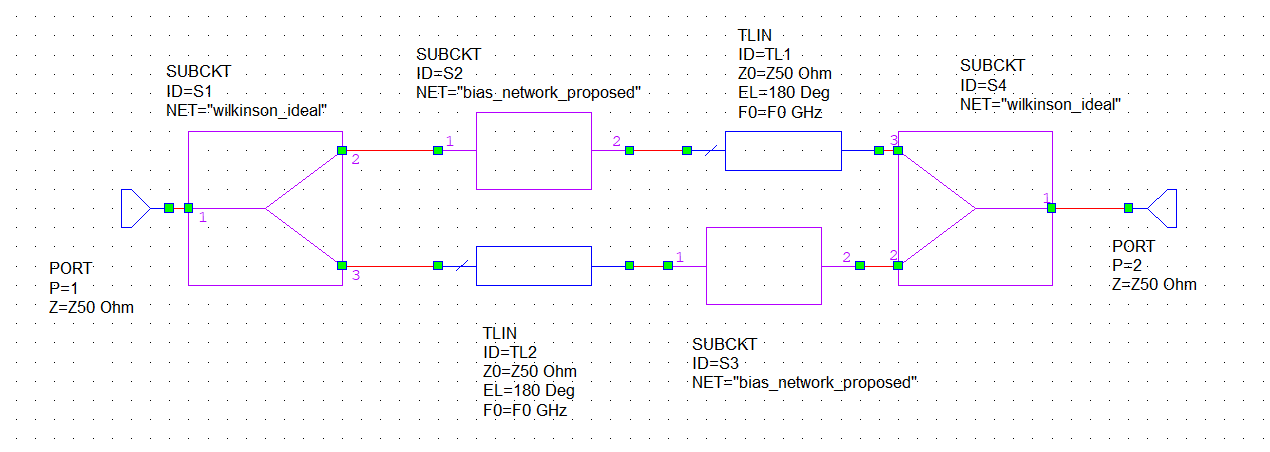
\includegraphics[width=1\linewidth]{images//design_circuit_elements/balanced_amplifier_ideal_circuit.png}
    \caption{Ideal balanced amplifier circuit}
    \label{fig:design_circuit_elements:balanced_amplifier_ideal_circuit}
\end{figure}

\begin{figure}
    \centering
    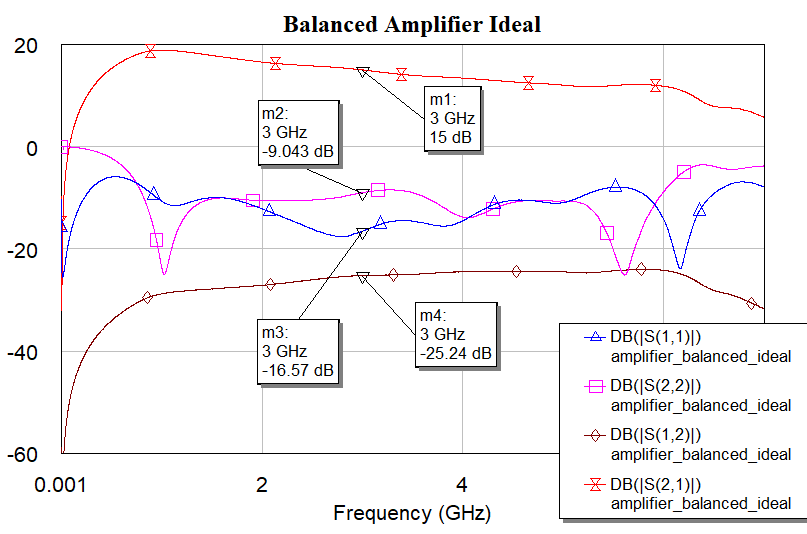
\includegraphics[width=1\linewidth]{images//design_circuit_elements/balanced_amplifier_ideal_graph.png}
    \caption{Simulation of the ideal balanced amplifier (see Figure \ref{fig:design_circuit_elements:balanced_amplifier_ideal_circuit})}
    \label{fig:design_circuit_elements:balanced_amplifier_ideal_graph}
\end{figure}

\section{Band Pass Filter}

\subsection{Filter order from the bandwidth, in-band return loss and the minimum attenuation at the stop bands}

Given the following values in the Figure \ref{fig:introduction:initial_parameters}:

\begin{align*}
\text{Center frequency} & : f_0 = 3 GHz\\
\text{Pass band lower limit} & : f_{p1} = 2.925 GHz\\
\text{Pass band upper limit} & : f_{p2} = 3.075 GHz\\
\text{Lower attenuation band limit} & : f_{a1} = 2.85 GHz\\
\text{Upper attenuation band limit} & : f_{a2} = 3.15 GHz\\
\end{align*}

Where:
\begin{align*}
w'_{p1} &= 2 \* \pi \* f'_{p1} = 2 \* \pi \* 2.925 \cdot 10^9 = 1.838 \cdot 10^{10} rad/s \\
w'_{p2} &= 2 \* \pi \* f'_{p2} = 2 \* \pi \* 3.075 \cdot 10^9 = 1.932 \cdot 10^{10} rad/s \\
w'_{a1} &= 2 \* \pi \* f'_{a1} = 2 \* \pi \* 2.85 \cdot 10^9 = 1.791 \cdot 10^{10} rad/s \\
w'_{a2} &= 2 \* \pi \* f'_{a2} = 2 \* \pi \* 3.15 \cdot 10^9 = 1.979 \cdot 10^{10} rad/s \\
\end{align*}

And also, we have a requirement of a minimum attenuation of 25 dB. Therefore, we will be choosing an attenuation of $\alpha_{a} = 30 dB$ to be sure that the filter works correctly. As we want the input losses to be bigger than $20 dB$ then:

\begin{align*}
s_{11} >= 30 dB \Rightarrow s_{11} &= 30 dB \\
s_{11} &= 10^{\frac{-30}{20}} = 0.032
\end{align*}

Now that we have the return loss, we can calculate the maximum transmission loss (or better said the maximum pass band attenuation). As we want our filter to be lossless, then $s_{11}^2 + s_{12}^2 = 1$. With this formula and the previous value we calculated, we can get the following:

\begin{align*}
\alpha_{p} &= - 20 \* \log_{10}(s_{12}) \\
&= \-20 \* \log_{10}(\sqrt{1 - s_{11}^2}) \\
&= \-20 \* \log_{10}(\sqrt{1 - 0.032^2}) \\
&= 4.45 \cdot 10^{-3} dB
\end{align*}

Now with the attenuation at each stage, the bandwidth of our filter is:

\begin{align*}
B &= \frac{(w'_{p2} - w'_{p1})}{w_p} = \frac{1.932 \cdot 10^{10} - 1.838 \cdot 10^{10}}{1} \\
&= 9.4 \cdot 10^{8} rad/s \\
\end{align*}

Where:
\begin{align*}
w_p &= 1 rad/s \text{ as it is the normalized angular frequency}
\end{align*}

And finally, we can calculate the filter order of our design by:

\begin{align*}
N &\geq \frac{\cosh^{-1}{1/k_d}}{\cosh^{-1}{1/k_s}} \\
&\geq \frac{\cosh^{-1}{1/1.013 \cdot 10^{-3}}}{\cosh^{-1}{1/0.509}} \\
&\geq 5.853 \Rightarrow N = 6
\end{align*}

Where:
\begin{align*}
w_0^2 &= w'_{p2} \* w'_{p1} = 1.932 \cdot 10^{10} \cdot 1.838 \cdot 10^{10} \\
&= 3.551 \cdot 10^{20} \ (rad/s)^2 \\
w_{a1} &= \frac{((w'_{a1})^2 - w_{0}^2)}{B \* w'_{a1}} = \frac{(1.791 \cdot 10^{10})^2 - 3.551 \cdot 10^{20}}{9.4 \cdot 10^8 \cdot 1.791 \cdot 10^{10}} \\
&= -2.029 \\
w_{a2} &= \frac{((w'_{a2})^2 - w_{0}^2)}{B \* w'_{a2}} = \frac{(1.979 \cdot 10^{10})^2 - 3.551 \cdot 10^{20}}{9.4 \cdot 10^8 \cdot 1.979 \cdot 10^{10}} \\
&= 1.964 \\
w_a &= \min (|w_{a1} |, |w_{a2}|) = \min (2.029, 1.964) \\
&= 1.964 \\
k_s &= \frac{w_p}{w_a} = \frac{1}{1.964} \\
&= 0.509 \\
k_d &= \sqrt{\frac{1 - 10^{\alpha_p / 10}}{1 - 10^{\alpha_a / 10}}} = \sqrt{\frac{1 - 10^{4.45 \cdot 10^{-3} / 10}}{1 - 10^{30 / 10}}} \\
&= 1.013 \cdot 10^{-3}
\end{align*}

\subsection{Parameters of the frequency and impedance transforms}

For the parameters, there were calculate before in order to get the filter order. We get a center pulsation of $w_0 = 1.8844 \cdot 10^{10} rad/s = 3 GHz$ as expected and a bandwidth of $B = 9.4 \cdot 10^{9} rad/s = 0.15 GHz$; which correspond to the requirements of the filter.

\subsection{Calculations of the normalized elements of the Chebyshev filter}

To calculate the coefficients of the Chebyshev filter with order 6, we will be using the calculator found in Aula Global. In our case, as the requirements for the return losses are that it must be at least 18 dB, we will be using an attenuation of 25 dB. See Figure \ref{fig:design_circuit_elements:chebyshev_filter_normalized_elements_calculator} to see the coefficients we will be using for the normalized elements ($g_i$). 

Here are the values that we will be using:
\begin{align*}
g_1 &= 0.820541 \\
g_2 &= 1.376845 \\
g_3 &= 1.728513 \\
g_4 &= 1.544460 \\
g_5 &= 1.540923 \\
g_6 &= 0.733169 \\
g_7 &= 1.119170 \\
\end{align*}

\begin{figure}
    \centering
    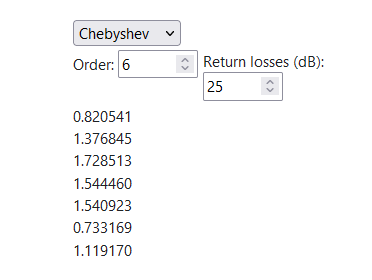
\includegraphics[width=1\linewidth]{images//design_circuit_elements/chebyshev_filter_normalized_elements_calculator.png}
    \caption{Calculations of the Chebyshev coefficients using the Aula Global calculator}
    \label{fig:design_circuit_elements:chebyshev_filter_normalized_elements_calculator}
\end{figure}

\subsection{Calculations of the inverters and even and odd impedances of the couple lines}

In order to calculate the inverters ($J_i$), we will use a bandwidth of $\Delta = 5\%$ as stated in the requirements. So let's calculate the inverters for the pass band filter to be able to implemented as a series of coupled lines. Note that as our filter order is 6, we will be using $6 + 1 = 7$ coupled lines.

\begin{align*}
J_1 \cdot Z_0 &= \sqrt{\frac{\pi \* \Delta}{2 \* g_1}} = \sqrt{\frac{\pi \cdot 0.05}{2 \cdot 0.820541}} = 0.30938 \\
J_2 \cdot Z_0 &= \frac{\pi \* \Delta}{2 \cdot \sqrt{g_1 \cdot g_2}} = \frac{\pi \cdot 0.05}{2 \cdot \sqrt{0.820541 \cdot 1.376845}} = 0.07389 \\
J_3 \cdot Z_0 &= \frac{\pi \* \Delta}{2 \cdot \sqrt{g_2 \cdot g_3}} = \frac{\pi \cdot 0.05}{2 \cdot \sqrt{1.376845 \cdot 1.728513}} = 0.05091 \\
J_4 \cdot Z_0 &= \frac{\pi \* \Delta}{2 \cdot \sqrt{g_3 \cdot g_4}} = \frac{\pi \cdot 0.05}{2 \cdot \sqrt{1.728513 \cdot 1.544460}} = 0.048069 \\
J_5 \cdot Z_0 &= \frac{\pi \* \Delta}{2 \cdot \sqrt{g_4 \cdot g_5}} = \frac{\pi \cdot 0.05}{2 \cdot \sqrt{1.544460 \cdot 1.540923}} = 0.050911 \\
J_6 \cdot Z_0 &= \frac{\pi \* \Delta}{2 \cdot \sqrt{g_5 \cdot g_6}} = \frac{\pi \cdot 0.05}{2 \cdot \sqrt{1.540923 \cdot 0.733169}} = 0.073892 \\
J_7 \cdot Z_0 &= \sqrt{\frac{\pi \* \Delta}{2 \cdot g_6 \cdot g_7}} = \sqrt{\frac{\pi \cdot 0.05}{2 \cdot 0.733169 \cdot 1.119170}} = 0.309382 \\
\end{align*}

And now we calculate the even and odd impedances of the coupled lines:

\begin{align*}
Z_{0e1} &= Z_0 \cdot (1 + J_1 \cdot Z_0 + (J_1 \cdot Z_0)^2) = 50 \cdot (1 + 0.30938 + (0.30938)^2) = 70.255\Omega \\
Z_{0o1} &= Z_0 \cdot (1 - J_1 \cdot Z_0 + (J_1 \cdot Z_0)^2) = 50 \cdot (1 - 0.30938 + (0.30938)^2) = 39.317\Omega \\
Z_{0e2} &= Z_0 \cdot (1 + J_2 \cdot Z_0 + (J_2 \cdot Z_0)^2) = 50 \cdot (1 + 0.07389 + (0.07389)^2) = 53.967\Omega \\
Z_{0o2} &= Z_0 \cdot (1 - J_2 \cdot Z_0 + (J_2 \cdot Z_0)^2) = 50 \cdot (1 - 0.07389 + (0.07389)^2) = 46.578\Omega \\
Z_{0e3} &= Z_0 \cdot (1 + J_3 \cdot Z_0 + (J_3 \cdot Z_0)^2) = 50 \cdot (1 + 0.05091 + (0.05091)^2) = 52.675\Omega \\
Z_{0o3} &= Z_0 \cdot (1 - J_3 \cdot Z_0 + (J_3 \cdot Z_0)^2) = 50 \cdot (1 - 0.05091 + (0.05091)^2) = 47.584\Omega \\
Z_{0e4} &= Z_0 \cdot (1 + J_4 \cdot Z_0 + (J_4 \cdot Z_0)^2) = 50 \cdot (1 + 0.048069 + (0.048069)^2) = 52.519\Omega \\
Z_{0o4} &= Z_0 \cdot (1 - J_4 \cdot Z_0 + (J_4 \cdot Z_0)^2) = 50 \cdot (1 - 0.048069 + (0.048069)^2) = 47.712\Omega \\
Z_{0e5} &= Z_0 \cdot (1 + J_5 \cdot Z_0 + (J_5 \cdot Z_0)^2) = 50 \cdot (1 +  0.050911 + ( 0.050911)^2) = 52.675\Omega \\
Z_{0o5} &= Z_0 \cdot (1 - J_5 \cdot Z_0 + (J_5 \cdot Z_0)^2) = 50 \cdot (1 -  0.050911 + ( 0.050911)^2) = 47.584\Omega \\
Z_{0e6} &= Z_0 \cdot (1 + J_6 \cdot Z_0 + (J_6 \cdot Z_0)^2) = 50 \cdot (1 + 0.073892 + (0.073892)^2) = 53.968\Omega \\
Z_{0o6} &= Z_0 \cdot (1 - J_6 \cdot Z_0 + (J_6 \cdot Z_0)^2) = 50 \cdot (1 - 0.073892 + (0.073892)^2) = 46.578\Omega \\
Z_{0e7} &= Z_0 \cdot (1 + J_7 \cdot Z_0 + (J_7 \cdot Z_0)^2) = 50 \cdot (1 + 0.309382 + (0.309382)^2) = 70.255\Omega \\
Z_{0o7} &= Z_0 \cdot (1 - J_7 \cdot Z_0 + (J_7 \cdot Z_0)^2) = 50 \cdot (1 - 0.309382 + (0.309382)^2) = 39.317\Omega \\
\end{align*}

\subsection{Simulation of the ideal band pass filter}

In order to simulate the band pass filter, we will implement it with ideal inverters first and then with ideal coupled lines. And after that we will compare the two and see if we get similar results.

In the Figure \ref{fig:design_circuit_elements:band_pass_filter_inverters_circuit}, we can see the circuit we implemented with inverters and the values calculated previously. If we check the simulation (see Figure \ref{fig:design_circuit_elements:band_pass_fitlter_inverters_graph}), we can see that the filter behaves correctly as the requirements stated. The attenuation at the pass band is less than 25 dB while the attenuation outside the attenuation band is more than 30 dB.

\begin{figure}[htbp]
    \centering
    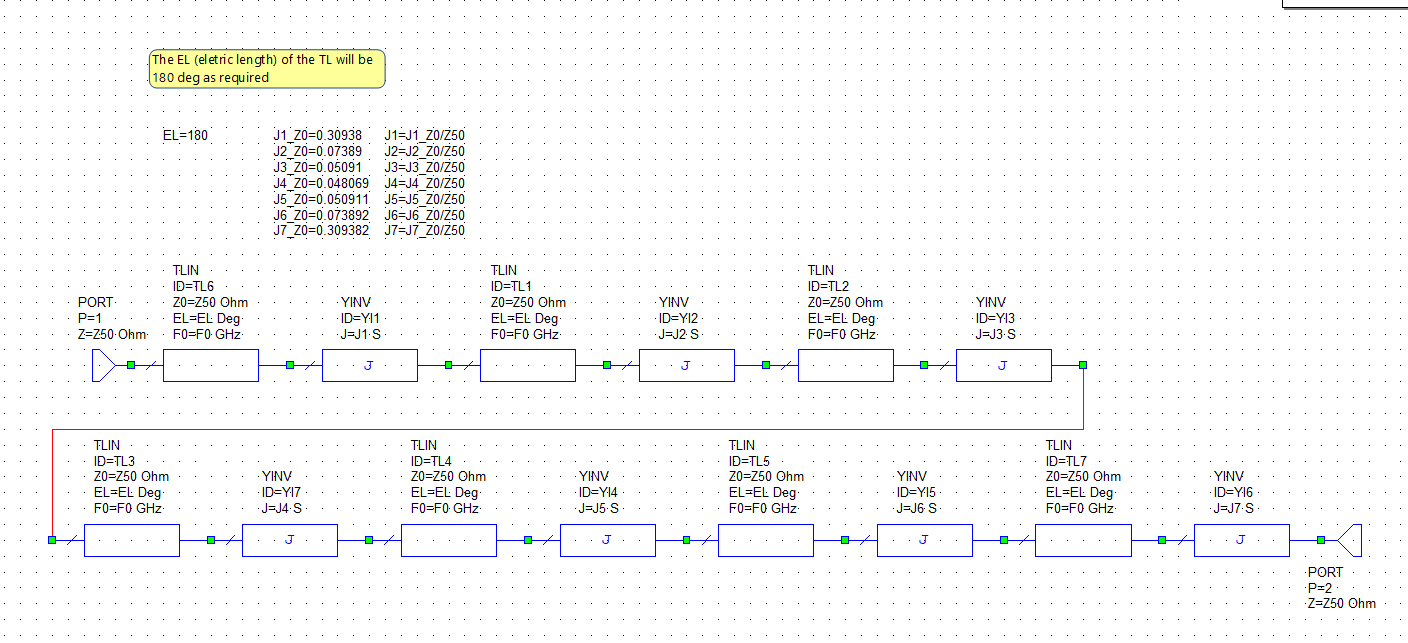
\includegraphics[width=1\linewidth]{images//design_circuit_elements/band_pass_filter_inverters_circuit.png}
    \caption{Circuit implementation of the band pass filter with inverters}
    \label{fig:design_circuit_elements:band_pass_filter_inverters_circuit}
\end{figure}

\begin{figure}[htbp]
    \centering
    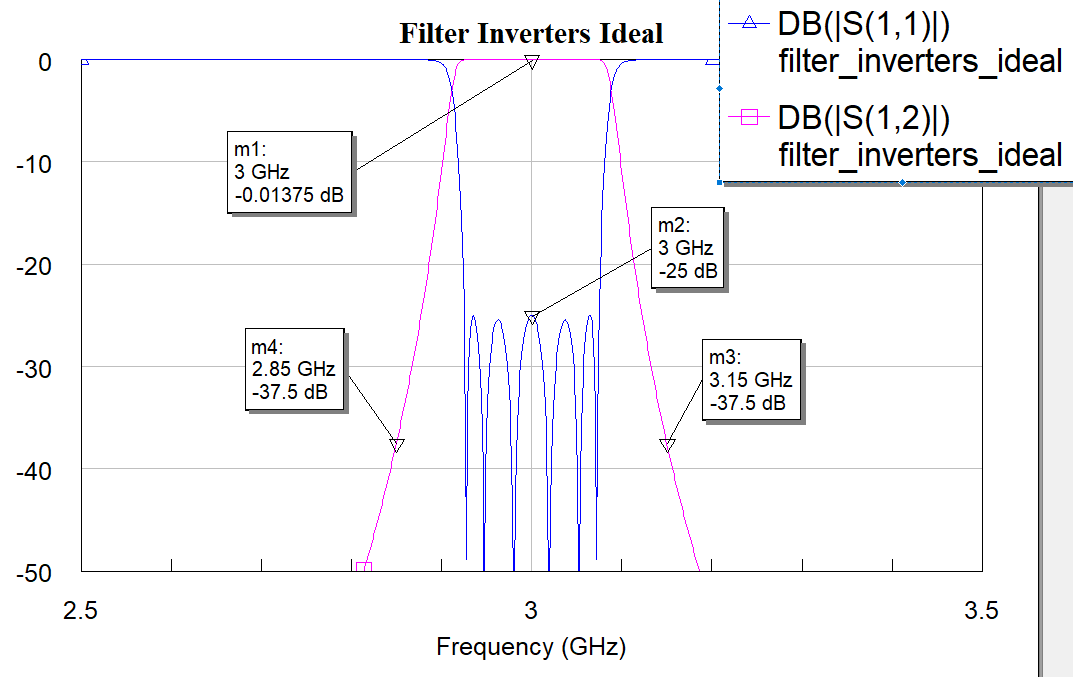
\includegraphics[width=1\linewidth]{images//design_circuit_elements/band_pass_fitlter_inverters_graph.png}
    \caption{Simulation of the band pass filter with inverters of Figure \ref{fig:design_circuit_elements:band_pass_filter_inverters_circuit}}
    \label{fig:design_circuit_elements:band_pass_fitlter_inverters_graph}
\end{figure}

Now, that we know that our coefficients are correctly calculated, we will implement the pass band filter with ideal coupled lines. For that we will be using the different even and odd impedances calculated previously. For the circuit shown in the Figure \ref{fig:design_circuit_elements:band_pass_filter_coupled_lines_ideal_circuit}, we get the simulation in Figure \ref{fig:design_circuit_elements:band_pass_filter_coupled_lines_ideal_graph}. In the simulation we can see that we get the same results as the filter implementation with inverters (see Figure \ref{fig:design_circuit_elements:band_pass_fitlter_inverters_graph}).

\begin{figure}[htbp]
    \centering
    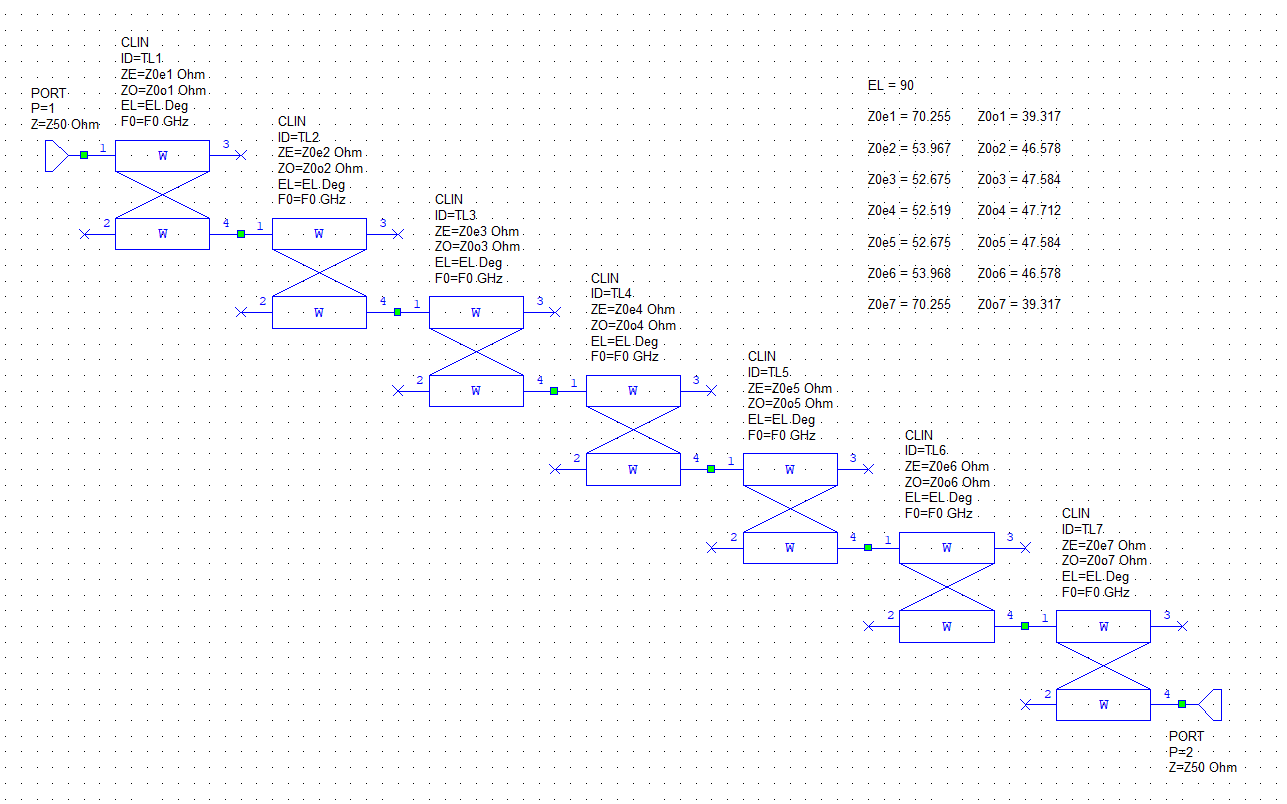
\includegraphics[width=1\linewidth]{images//design_circuit_elements/band_pass_filter_coupled_lines_ideal_circuit.png}
    \caption{Filter implementation with ideal coupled lines}
    \label{fig:design_circuit_elements:band_pass_filter_coupled_lines_ideal_circuit}
\end{figure}

\begin{figure}[htbp]
    \centering
    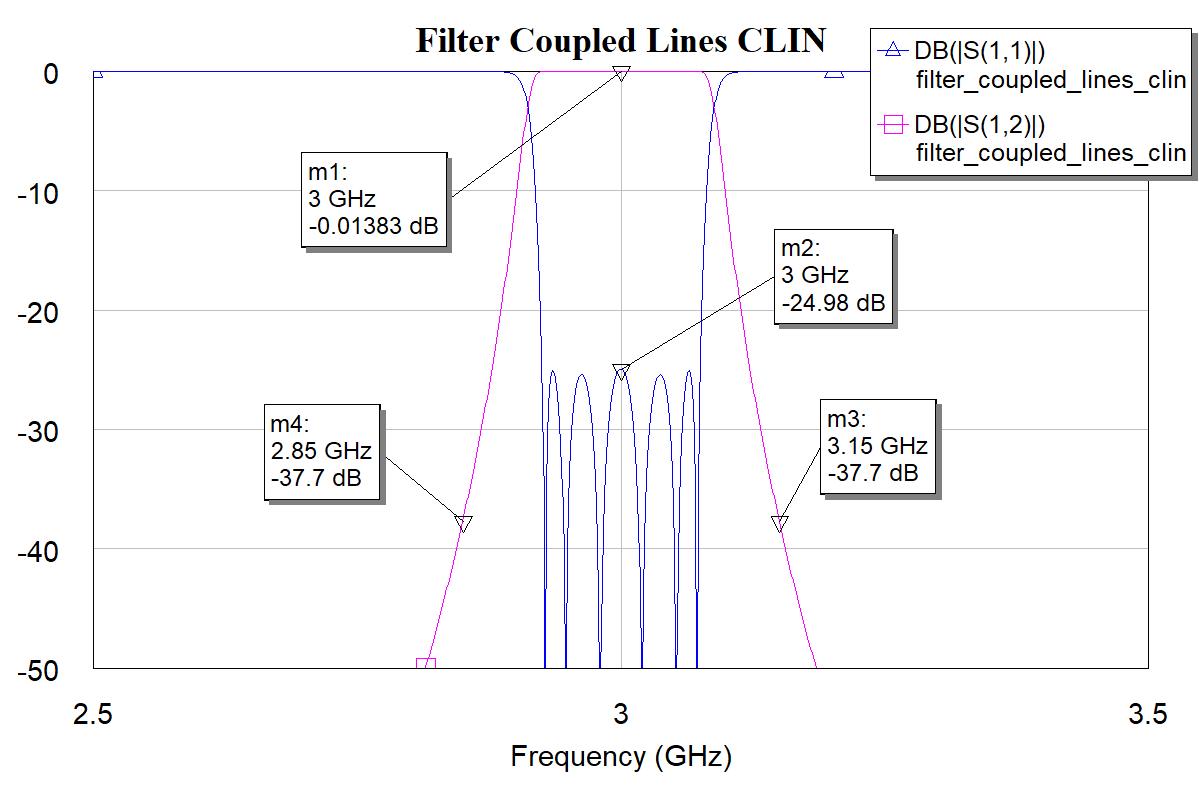
\includegraphics[width=1\linewidth]{images//design_circuit_elements/band_pass_filter_coupled_lines_ideal_graph.png}
    \caption{Simulation of the filter implementation with ideal coupled lines (see Figure \ref{fig:design_circuit_elements:band_pass_filter_coupled_lines_ideal_circuit})}
    \label{fig:design_circuit_elements:band_pass_filter_coupled_lines_ideal_graph}
\end{figure}

\section{Directional Coupler}

In order to measure the signal and check the correct functionality, we will be using a directional coupler. Let's start with the study of the element.

\subsection{Electrical length and even and odd characteristic impedances of the couple-line section}

According to the requirements of the system, the power at the monitor port must be 20 dB below the main line. That means that the coupling of the directional amplifier must be $C_{dB} = 20 dB$.

\begin{align*}
C &= 10^{\frac{- C_{dB}}{10}} \\
&= 10^{\frac{- 20}{10}} \\
&= 0.1 \\
\end{align*}

Now, in order to calculate the characteristic impedances of the even and odd modes, first we will assume an electrical length of $\lambda / 4$ or the same as $90 \deg$. That means that the coupler will be a symmetric coupler with a $90 \deg$ phase shift between the transmitted and the coupled port,

Given a electrical length of $\lambda / 4$, then we can use the following formulas to calculate the characteristic impedances of the even and odd modes, for the even mode we get:

\begin{align*}
Z_{0, even} &= Z_{0} \* \sqrt{\frac{1 + C}{1 - C}} \\
&= 55.28 \Omega \\
\end{align*}

And for the odd mode:

\begin{align*}
Z_{0, odd} &= Z_{0} \* \sqrt{\frac{1 - C}{1 + C}} \\
&= 45.23 \Omega \\
\end{align*}

\subsection{Connection of the coupler}

For this coupler, the main objective is to transmit the whole power entering from the input to the transmitted and coupled ports. For this case, we want the following scattering parameter matrix:

\[
S = \begin{bmatrix}
0 & \alpha & j \* \beta & 0 \\
\alpha & 0 & 0 & j \* \beta \\
j \* \beta & 0 & 0 & \alpha \\
0 & j \* \beta & \alpha & 0 \\
\end{bmatrix}
\]

Where:
\begin{align*}
& \text{We assume an isolation of $I = \infty \ dB$}  \\
& \text{Port 1 is the input port} \\
& \text{Port 2 is the coupled port} \\
& \text{Port 3 is the transmission port} \\
& \text{Port 4 is the isolated port} \\
\end{align*}

Usually for a directed port, you want that the isolated port is degenerated with respect to the other 3. Therefore, we will be loading it with a matched load, that is equal to the characteristic impedance of $Z_0 = 50 \Omega$. You can see the final circuit for the directed coupler in Figure \ref{fig:design_circuit_elements:directional_coupler_ideal_circuit}.

\begin{figure}[htbp]
    \centering
    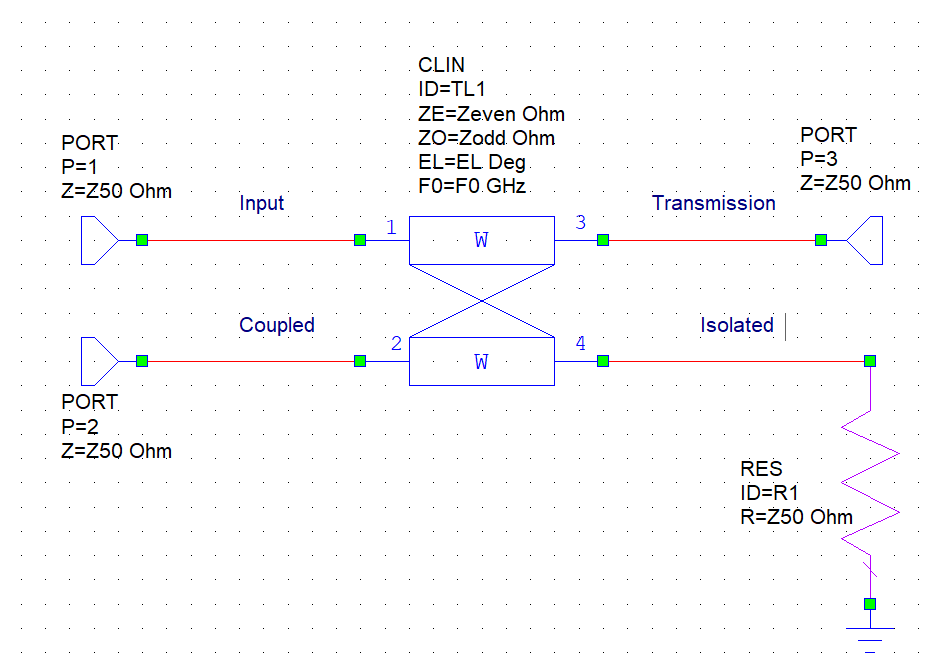
\includegraphics[width=\textwidth]{images/design_circuit_elements/directional_coupler_ideal_circuit.png}
    \caption{Ideal circuit for the directional coupler}
    \label{fig:design_circuit_elements:directional_coupler_ideal_circuit}
\end{figure}

If we simulate the circuit with AWR (see Figure \ref{fig:design_circuit_elements:directional_coupler_ideal_graph}), we can see that there is no reflection at the input port as the $s_{11} = -84 \ dB$, the coupling is $C = -20 \ dB$ as expected, and the rest of the power is directed to the transmission port.

\begin{figure}[htbp]
    \centering
    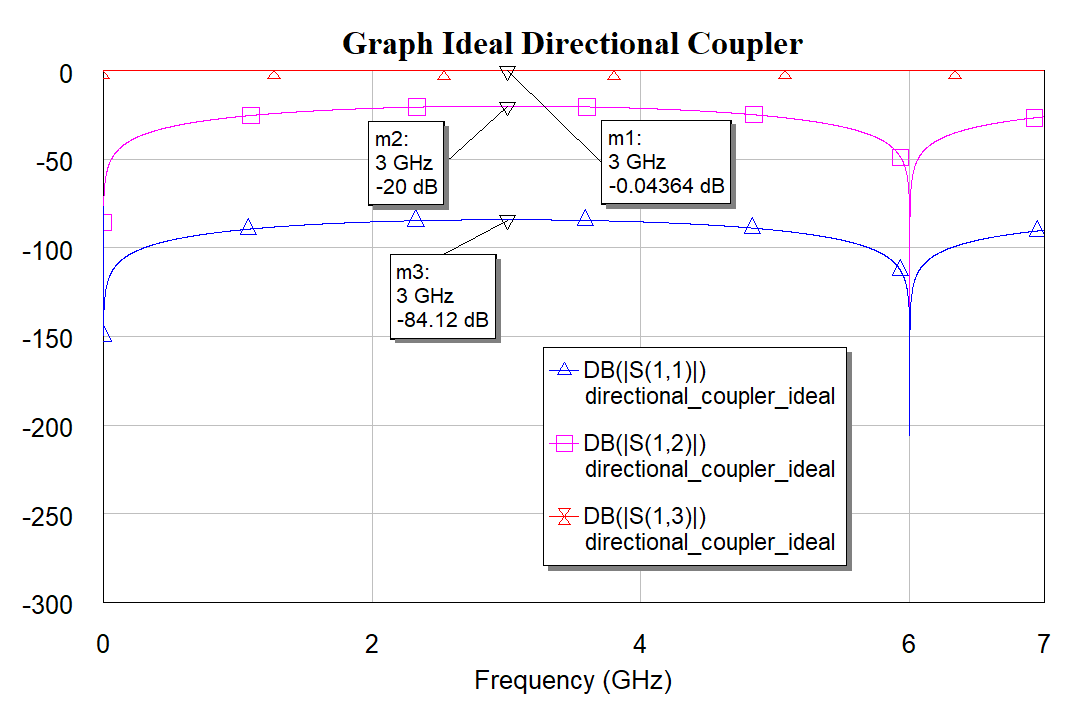
\includegraphics[width=\linewidth]{images//design_circuit_elements/directional_coupler_ideal_graph.png}
    \caption{Simulation of the ideal directed coupler of Figure \ref{fig:design_circuit_elements:directional_coupler_ideal_circuit}}
    \label{fig:design_circuit_elements:directional_coupler_ideal_graph}
\end{figure}

%-----------------------------------------------------------
\chapter{Design and Characterization of the Microstrip Elements}

\section{Wilkinson Power Divider / Combiner}

In order to divide the input signal from the simple amplifier into to equal signals and then join the signals together after they have been amplified in the second stage, we will be using a Wilkinson divider / combiner.

\subsection{Ideal Wilkinson Power Divider / Combiner}

First we have designed an ideal Wilkinson divider / combiner (see Figure \ref{fig:microstrip_elements:wilkinson_ideal_circuit}). We have used a resistance of $R = 2 \* Z_0 = 100 \Omega$ for the resistance between the two output ports. And also a characteristic impedance of the lines of $Z_{0,W} = \sqrt{2} \* Z_0 \ \Omega = 70.71 \ \Omega$.

\begin{figure}[htbp]
    \centering
    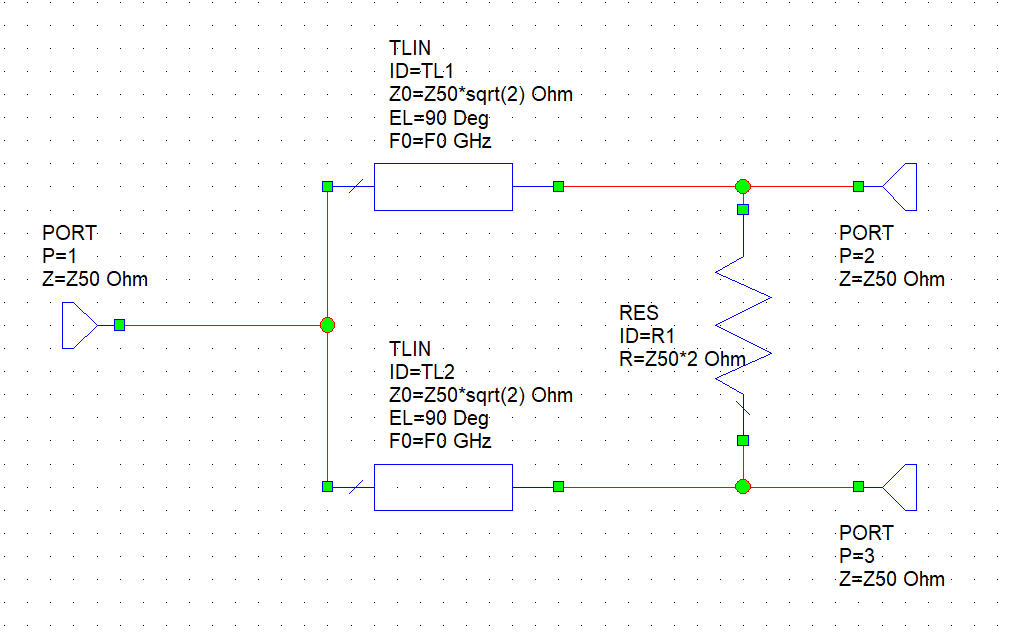
\includegraphics[width=\linewidth]{images/microstrip_elements/wilkinson_ideal_circuit.png}
    \caption{Ideal Wilkinson power divider / combiner circuit}
    \label{fig:microstrip_elements:wilkinson_ideal_circuit}
\end{figure}

If we simulate the circuit of Figure \ref{fig:microstrip_elements:wilkinson_ideal_circuit}, we get the following graph (see Figure \ref{fig:microstrip_elements:wilkinson_ideal_graph}). Here we can see that the reflected power is 0 as $s_{11} = - 249 dB$. And the transmitted power for each port is $s_{21} = s_{31} = 3 \ dB = 0.5$, that is half of the input power goes to each port.

\begin{figure}[htbp]
    \centering
    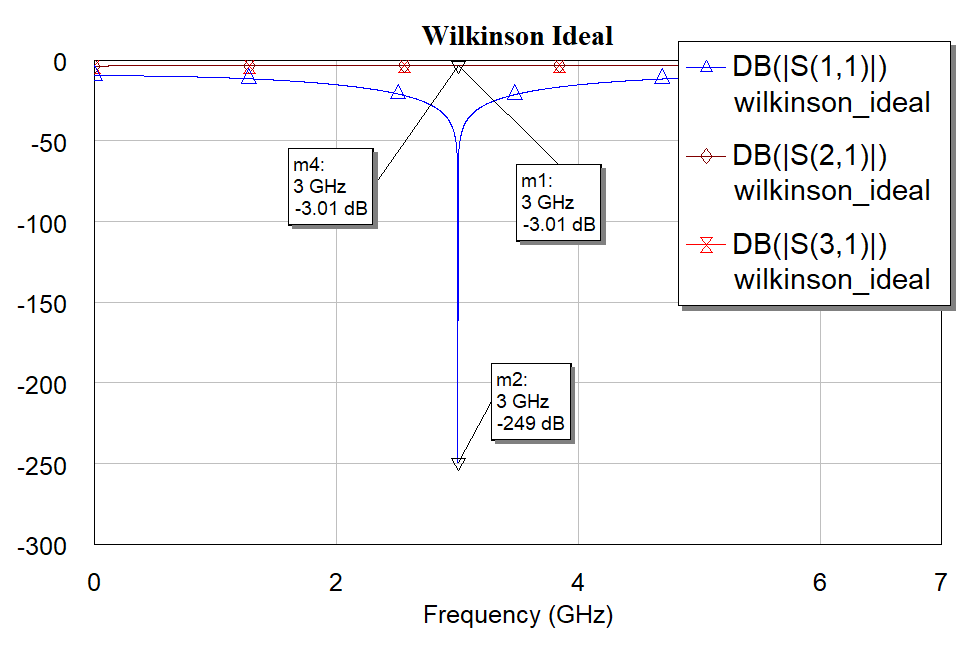
\includegraphics[width=1\linewidth]{images//microstrip_elements/wilkinson_ideal_graph.png}
    \caption{Simulation of an ideal Wilkinson power divider / combiner}
    \label{fig:microstrip_elements:wilkinson_ideal_graph}
\end{figure}

\subsection{Implementation with transmission lines}

In order to implement this in our design, we will have to adapt the ideal Wilkinson power divider / combiner to our circuit. For this we will have to calculate the width and length of the TLs for a characteristic impedance of $Z_{0,W} = 70.71 \ \Omega$. For this we have used the TXLine tool of AWR and we got a width of $w = 0.9065 mm$ and a height of $h = 12.19 mm$ (see Figure \ref{fig:microstrip_elements:wilkinson_real_txline_tool_calculations}).

\begin{figure}[htbp]
    \centering
    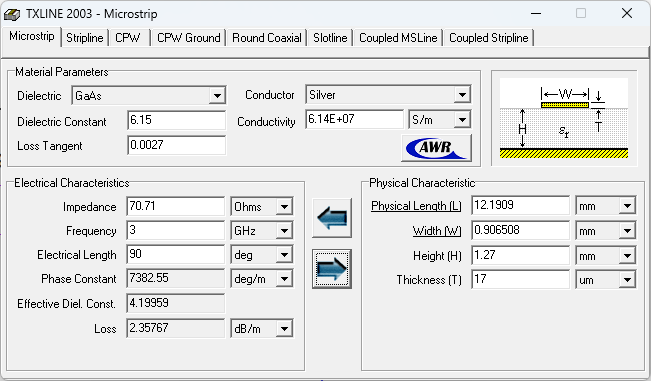
\includegraphics[width=1\linewidth]{images//microstrip_elements/wilkinson_real_txline_tool_calculations.png}
    \caption{Calculations of the width and height of the Wilkinson power divider / combiner}
    \label{fig:microstrip_elements:wilkinson_real_txline_tool_calculations}
\end{figure}

Now, if we simulate the following circuit with the TL with the correct dimensions (see Figure \ref{fig:microstrip_elements:wilkinson_real_circuit}), we get the graph shown in Figure \ref{fig:microstrip_elements:wilkinson_real_graph}.
Here we can observe that the implementation of the Wilkinson power divider / combiner works correctly as it divides the power in half and it has almost no reflection. However, this implementation is really difficult to implement in a microstrip line, so let's change the design to make it easier to implement.

\begin{figure}[htbp]
    \centering
    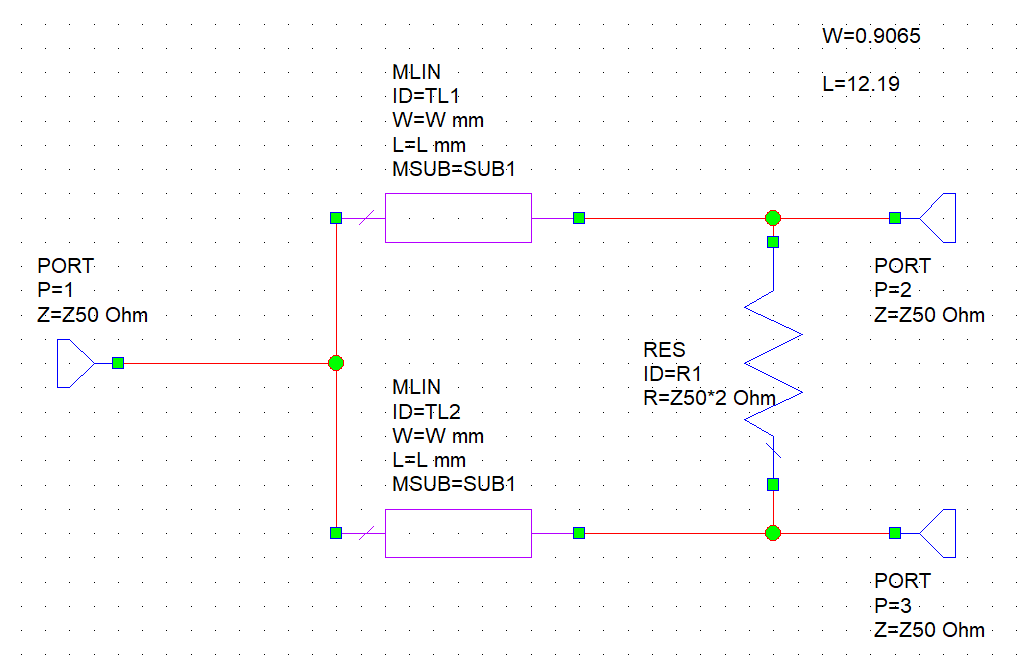
\includegraphics[width=1\linewidth]{images//microstrip_elements/wilkinson_real_circuit.png}
    \caption{Microstrip circuit design of the Wilkinson power divider / combiner}
    \label{fig:microstrip_elements:wilkinson_real_circuit}
\end{figure}

\begin{figure}[htbp]
    \centering
    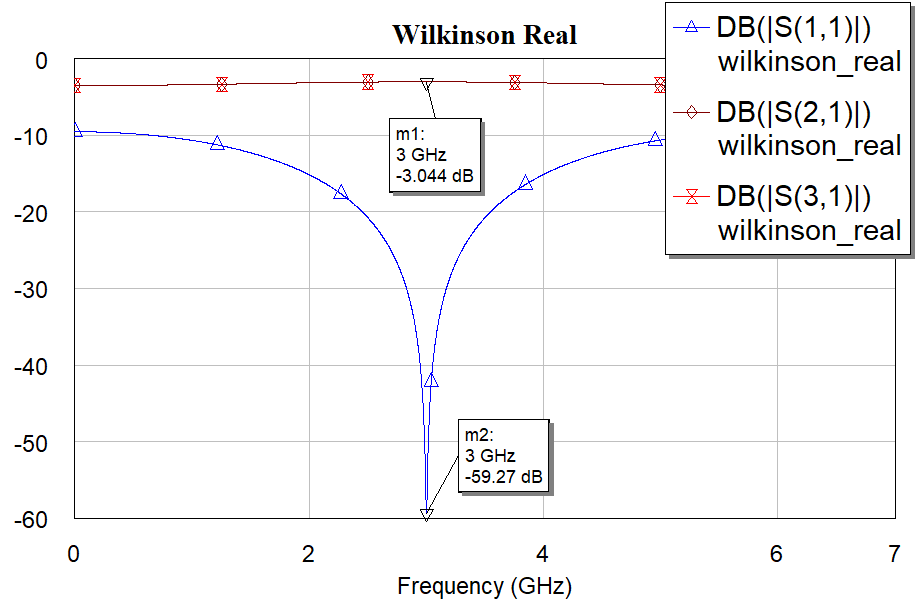
\includegraphics[width=1\linewidth]{images//microstrip_elements/wilkinson_real_graph.png}
    \caption{Simulation of the real Wilkinson power divider / combiner}
    \label{fig:microstrip_elements:wilkinson_real_graph}
\end{figure}

\subsection{Implementation with TEE junctions}

In order to incorporate the Wilkinson power divider / combiner in a microstrip technology, we will be using TEE junctions. For this implementation we will have to calculate the different radius shown in Figure \ref{fig:microstrip_elements:wilkinson_tee_design}. Note that the Gap will be the one required to solder the 0603 SMD resistor, for our case, we will be using $Gap = 1 mm$.

\begin{figure}
    \centering
    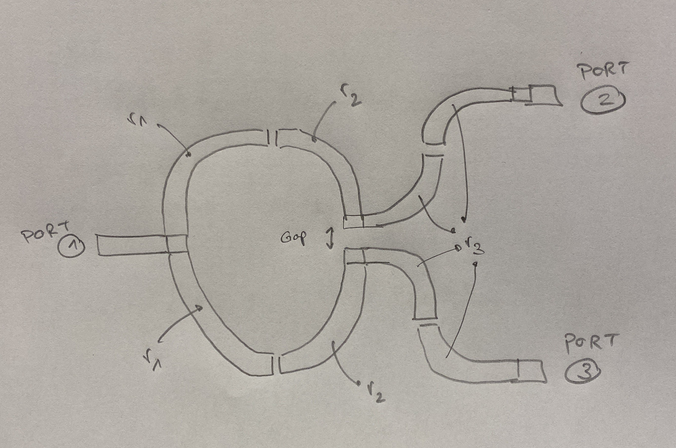
\includegraphics[width=1\linewidth]{images//microstrip_elements/wilkinson_tee_design.png}
    \caption{Design for the implementation of a Wilkinson with TEE junctions}
    \label{fig:microstrip_elements:wilkinson_tee_design}
\end{figure}

\begin{align*}
    r_1 &= \frac{1}{2} \* (\frac{\lambda}{2 \* \pi} + \frac{W_{50} + Gap}{2})  = \frac{1}{2} \* (\frac{c}{2 \* \pi \* f \* \sqrt{\epsilon_r}} + \frac{W_{50} + Gap}{2})  \\
    &= \frac{1}{2} \* (\frac{3 \cdot 10^8}{2 \* \pi \* 3 \cdot 10^9 \* \sqrt{6.15}} + \frac{1.85 \cdot 10^{-3} + 1 \cdot 10^{-3}}{2})  \\
    &= 4.031 \cdot 10^{-3} m = 4.031 mm \\
    \\
    r_2 &= r_1 - \frac{W_{50} + Gap}{2}  \\
    &= 4.031 \cdot 10^{-3} - \frac{1.85 \cdot 10^{-3} + 1 \cdot 10^{-3}}{2}  \\
    &= 2.606 \cdot 10^{-3} m = 2.606 mm \\
\end{align*}

Note: the width, $W_{50} = 1.85 mm$, we use is the one calculated in Figure \ref{fig:previous_work:duroid_6006_h_1_27_mm_50_ohm}.

And for $r_3$, we will be using a radius big enough so the amplifier stage fits in the balanced amplifier. For our case we will be using a radium of $r_3 = \lambda / 32 = 40.32 / 32 = 1.26 mm$.

In the Figure \ref{fig:microstrip_elements:wilkinson_microstrip_graph}, we can see the simulation of the Wilkinson power divider / combiner implemented in microstrip technology (see Figure \ref{fig:microstrip_elements:wilkinson_microstrip_circuit} to see the circuit implemented). Here we can observe that the theoretical calculations do not fit the requirement for our working frequency of $f_0 = 3 GHz$. Thus we will tune the circuit in order to adapt it for our working frequency using the AWR Tune Tool.

\begin{figure}[htbp]
    \centering
    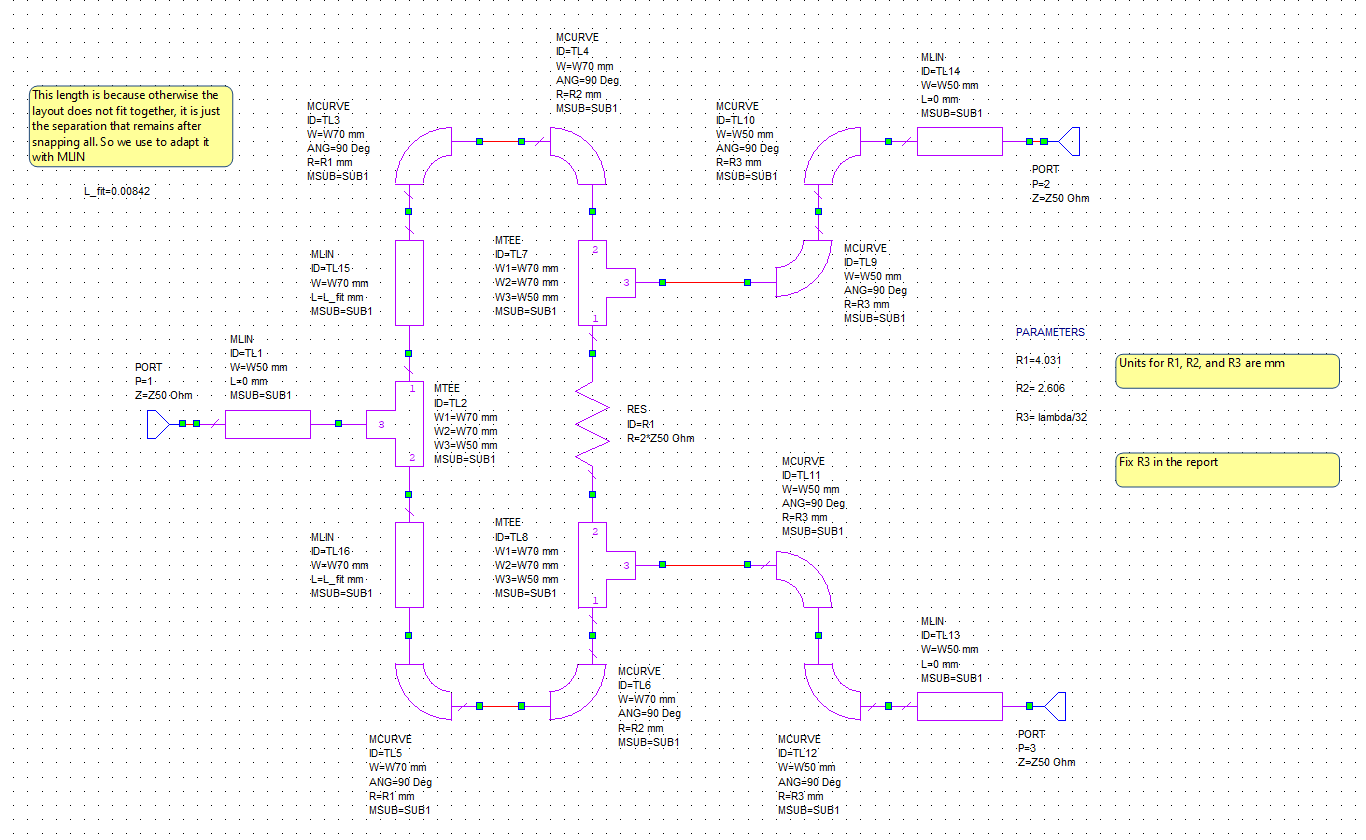
\includegraphics[width=1\linewidth]{images//microstrip_elements/wilkinson_microstrip_circuit.png}
    \caption{Wilkinson power divider / combiner circuit}
    \label{fig:microstrip_elements:wilkinson_microstrip_circuit}
\end{figure}

\begin{figure}[htbp]
    \centering
    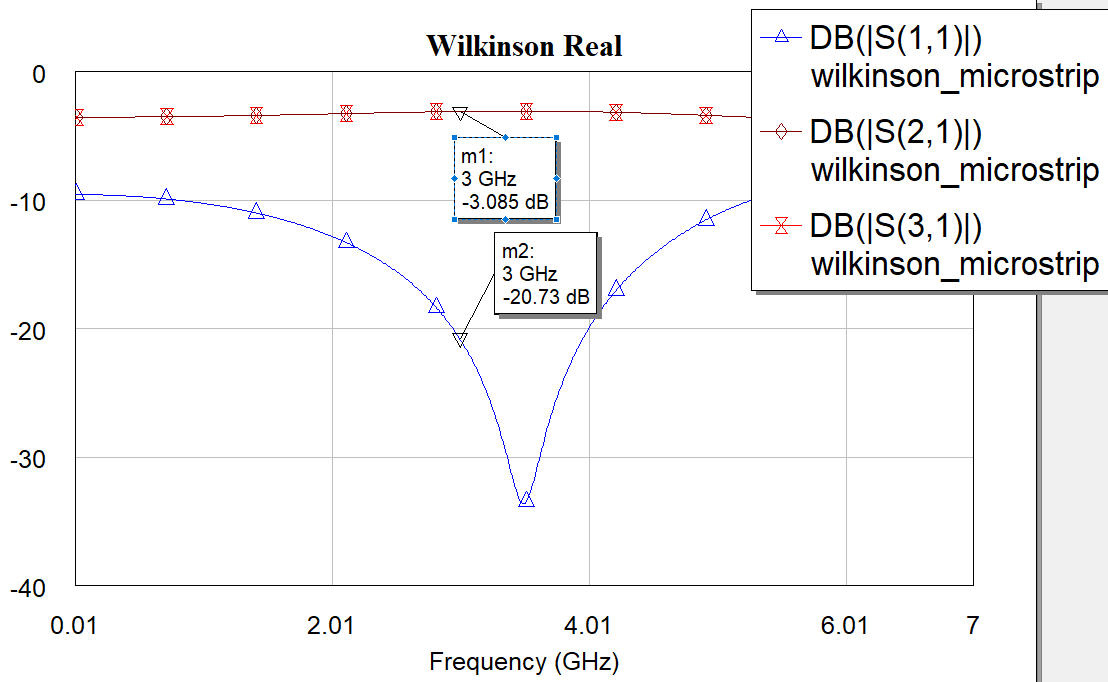
\includegraphics[width=1\linewidth]{images//microstrip_elements/wilkinson_microstrip_graph.png}
    \caption{Wilkinson power divider / combiner simulation of circuit in Figure \ref{fig:microstrip_elements:wilkinson_microstrip_circuit}}
    \label{fig:microstrip_elements:wilkinson_microstrip_graph}
\end{figure}

For the circuit tuned, we get slightly different values of $r_1 = 4.45mm$ and $r_2 = 3.35 mm$. For this we get the simulation shown in Figure \ref{fig:microstrip_elements:wilkinson_microstrip_tune_graph}, we can see that the Wilkinson is working perfectly. This is because the power is divided in half to the two output ports $s_{21}$ and $s_{31}$ and the reflection $s_{11}$ is negligible.

\begin{figure}[htbp]
    \centering
    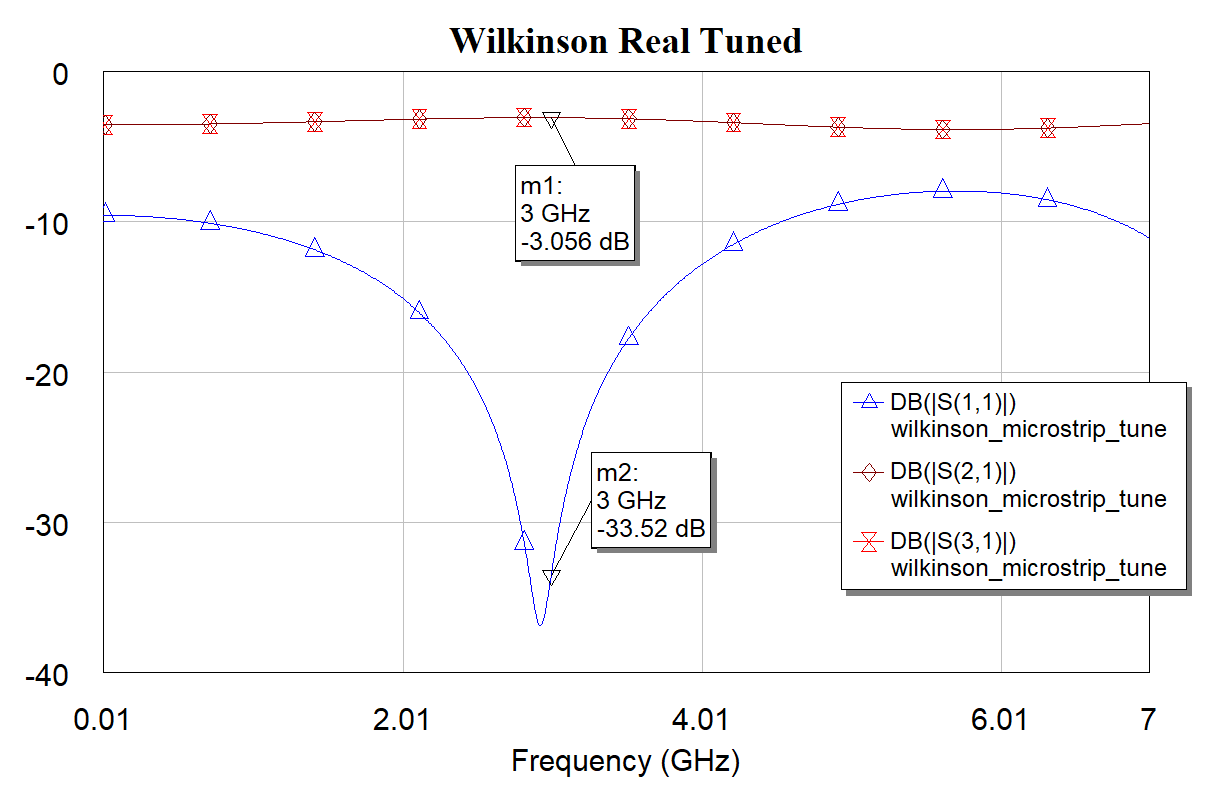
\includegraphics[width=1\linewidth]{images//microstrip_elements/wilkinson_microstrip_tune_graph.png}
    \caption{Simulation of the Wilkinson power divider / combiner tuned}
    \label{fig:microstrip_elements:wilkinson_microstrip_tune_graph}
\end{figure}

\subsection{Layout}

For the layout, we got the one show in Figure \ref{fig:microstrip_elements:wilkinson_microstrip_tune_layout}. One important note is that we added transmission lines at the junction between the input port and the two branches. The length was the one required for the layout to be able to snap together.

\begin{figure}[htbp]
    \centering
    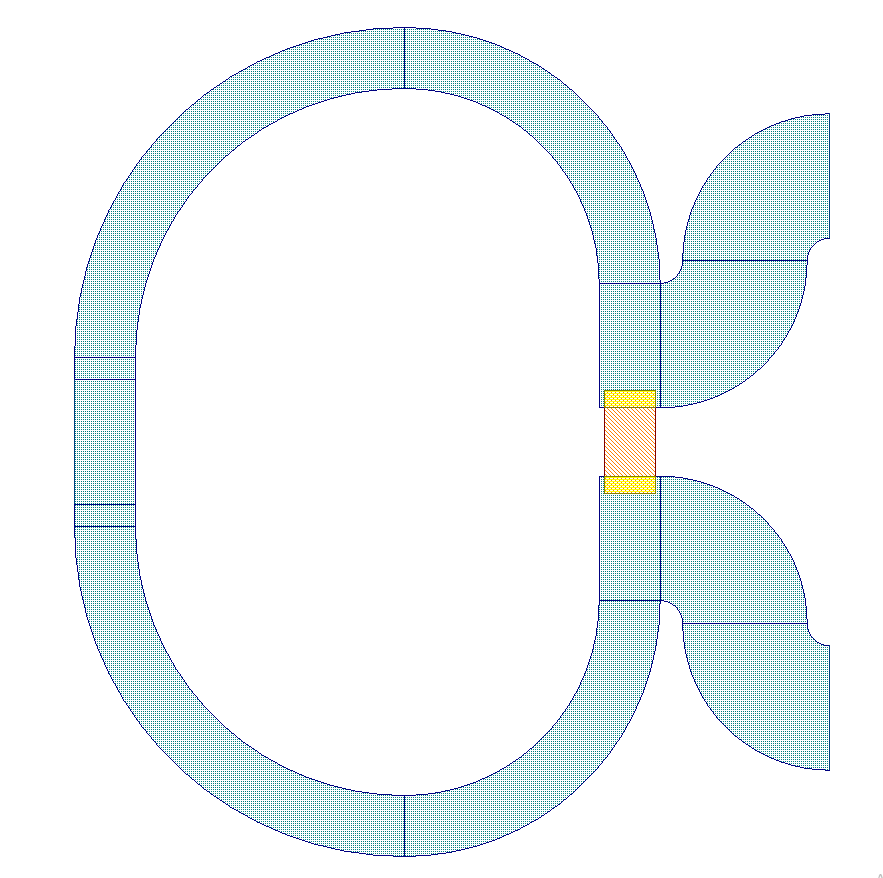
\includegraphics[width=1\linewidth]{images//microstrip_elements/wilkinson_microstrip_tune_layout.png}
    \caption{Layout of the Wilkinson power divider / combiner}
    \label{fig:microstrip_elements:wilkinson_microstrip_tune_layout}
\end{figure}

\section{First Stage: Simple Amplifier}

For the simple amplifier, we have implemented the circuit show in Figure \ref{fig:microstrip_elements:simple_amplifier_microstrip_circuit}. One thing to take into consideration, is that we have added small segments of transmission lines between the lumped elements so there is space for the layout design to be implemented.

\begin{figure}[htbp]
    \centering
    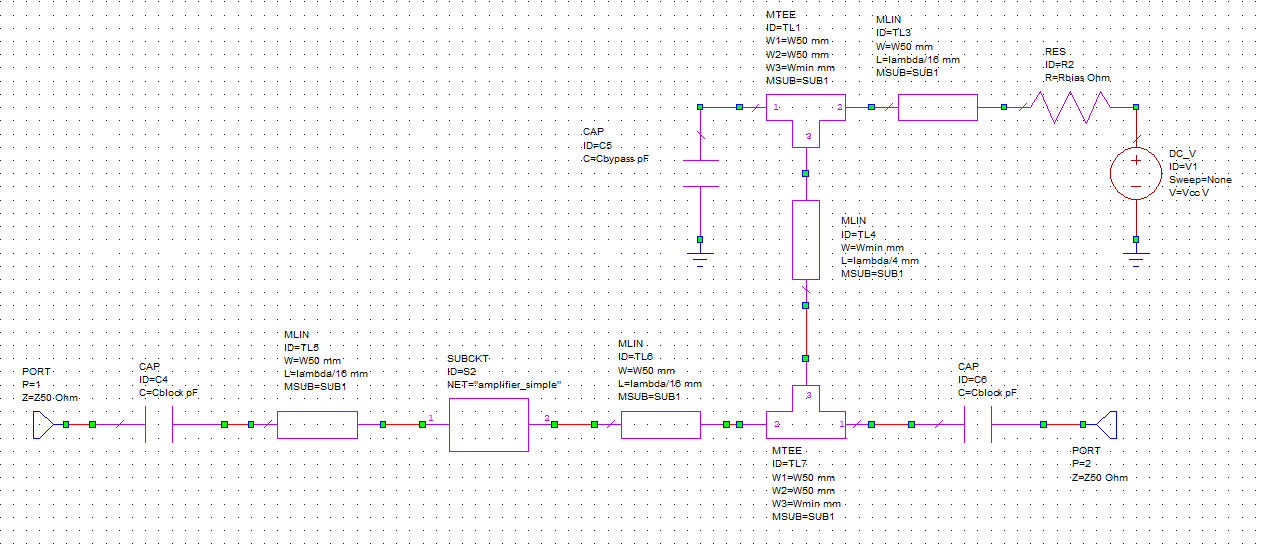
\includegraphics[width=1\linewidth]{images//microstrip_elements/simple_amplifier_microstrip_circuit.png}
    \caption{Circuit of first stage: simple amplifier}
    \label{fig:microstrip_elements:simple_amplifier_microstrip_circuit}
\end{figure}

The simulation for this circuit can be shown in Figure \ref{fig:microstrip_elements:simple_amplifier_microstrip_graph}. If we compare it with the data sheet of the amplifier (see Figure \ref{fig:design_circuit_elements:scattering_parameters_datasheet}), we can see that they are almost the same.

\begin{figure}[htbp]
    \centering
    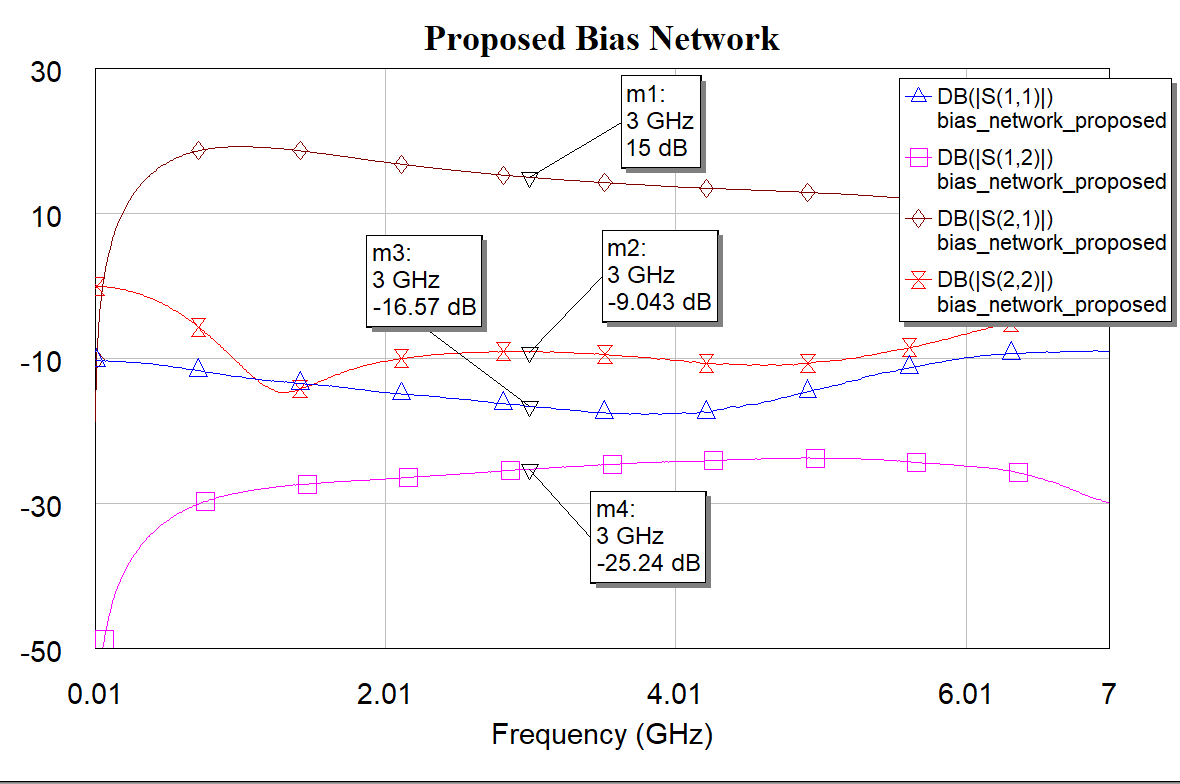
\includegraphics[width=1\linewidth]{images//microstrip_elements/simple_amplifier_microstrip_graph.png}
    \caption{Simulation of the first stage: simple amplifier show in Figure \ref{fig:microstrip_elements:simple_amplifier_microstrip_circuit}}
    \label{fig:microstrip_elements:simple_amplifier_microstrip_graph}
\end{figure}

\subsection{Layout}

Finally, the microstrip layout can be seen in Figure \ref{fig:microstrip_elements:simple_amplifier_microstrip_layout}.

\begin{figure}[htbp]
    \centering
    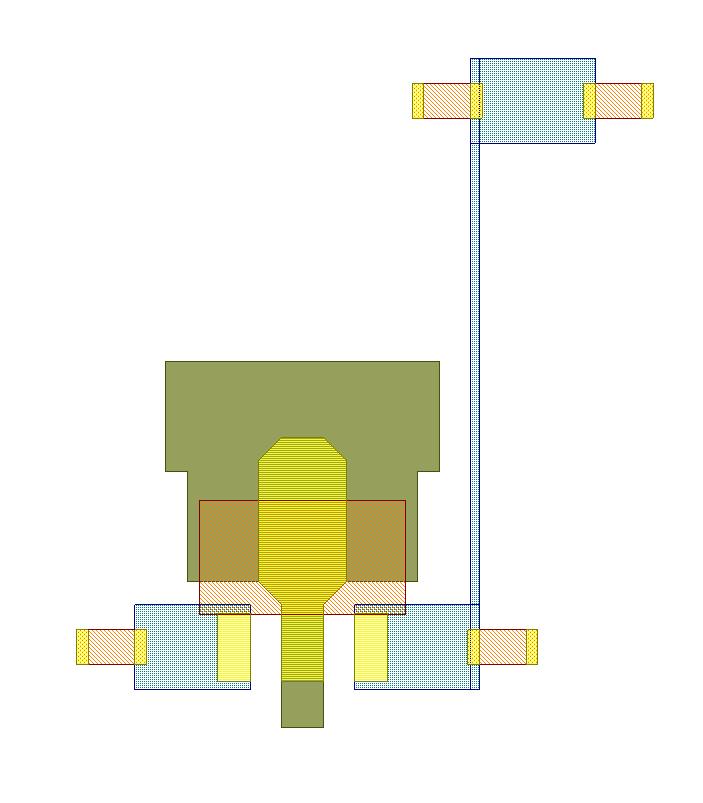
\includegraphics[width=1\linewidth]{images//microstrip_elements/simple_amplifier_microstrip_layout.png}
    \caption{Layout of the simple amplifier}
    \label{fig:microstrip_elements:simple_amplifier_microstrip_layout}
\end{figure}

\section{Second Stage: Balanced Amplifier}

For the second stage, we have implemented the circuit show in Figure \ref{fig:microstrip_elements:balanced_amplifier_microstrip_circuit}.  Here we have used the previous circuits such as the Wilkinson power divider / combiner and the bias network for the amplifier.

\begin{figure}[htbp]
    \centering
    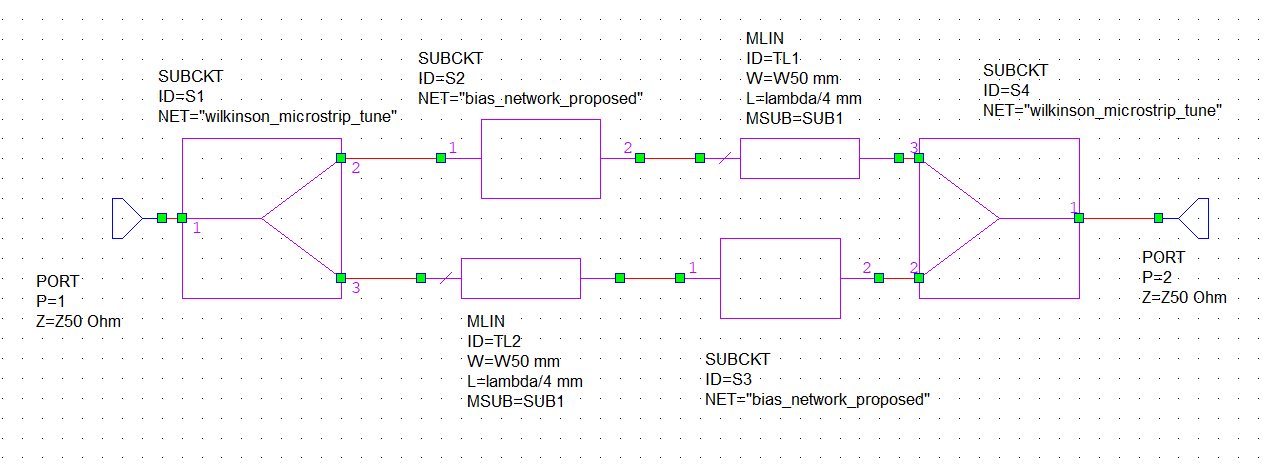
\includegraphics[width=1\linewidth]{images//microstrip_elements/balanced_amplifier_microstrip_circuit.png}
    \caption{Circuit of the balanced amplifier}
    \label{fig:microstrip_elements:balanced_amplifier_microstrip_circuit}
\end{figure}

If we compare the simulation of the balanced amplifier (see Figure \ref{fig:microstrip_elements:balanced_amplifier_microstrip_graph}) with the simulation for the simple amplifier (see Figure \ref{fig:microstrip_elements:simple_amplifier_microstrip_graph}); we can see that they have the same gain as calculated previously. However, the isolation of the balanced amplifier is much higher than the simple amplifier (as it has much lower $s_{11}$, $s_{12}$, and $s_{22}$. 

\begin{figure}[htbp]
    \centering
    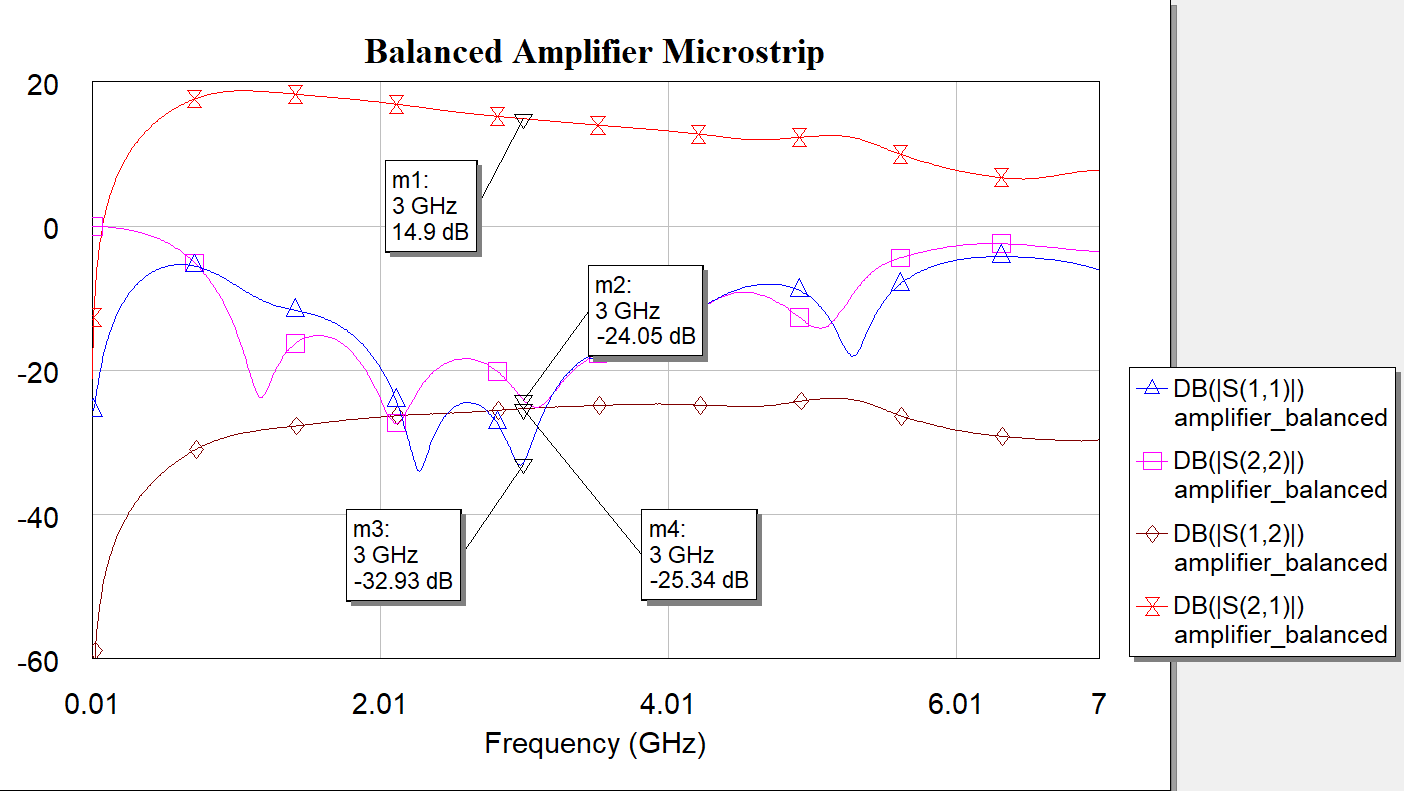
\includegraphics[width=1\linewidth]{images//microstrip_elements/balanced_amplifier_microstrip_graph.png}
    \caption{Simulation of the balanced amplifier in Figure \ref{fig:microstrip_elements:balanced_amplifier_microstrip_circuit}}
    \label{fig:microstrip_elements:balanced_amplifier_microstrip_graph}
\end{figure}

\subsection{Layout}

For the layout, it can be seen in Figure \ref{fig:microstrip_elements:balanced_amplifier_microstrip_layout}.

\begin{figure}[htbp]
    \centering
    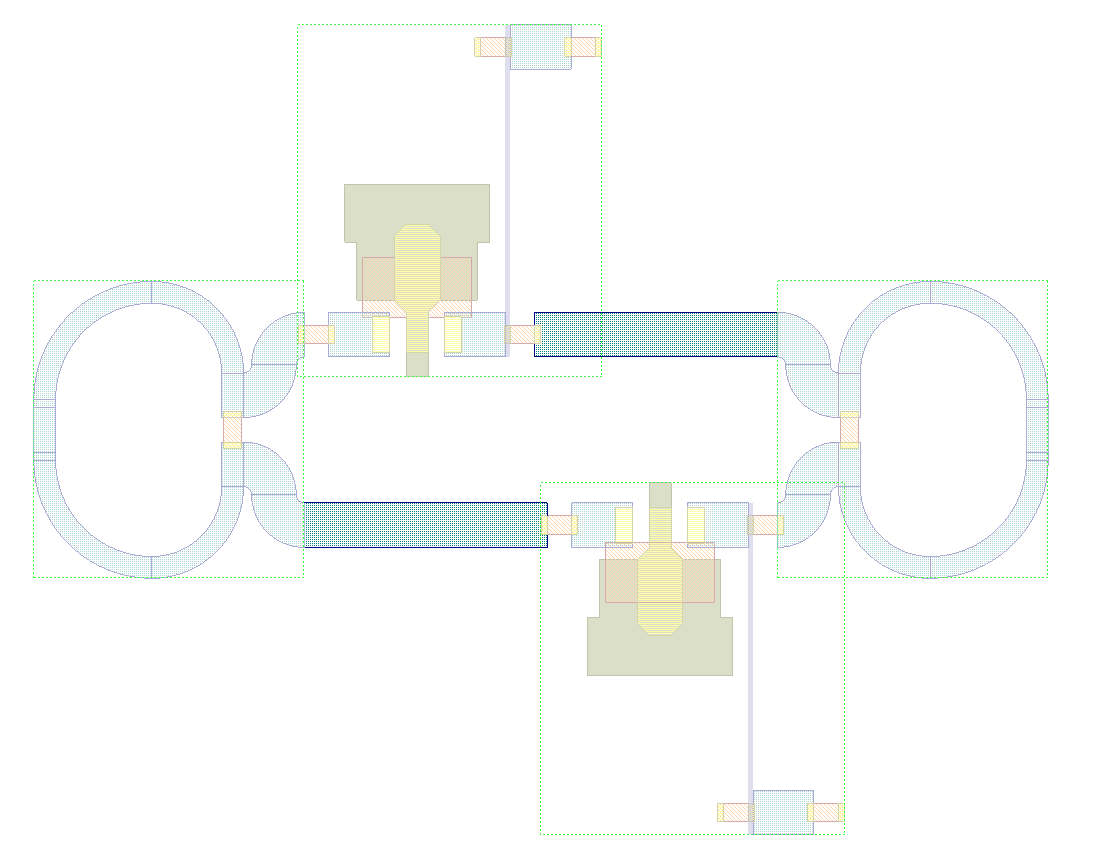
\includegraphics[width=1\linewidth]{images//microstrip_elements/balanced_amplifier_microstrip_layout.png}
    \caption{Layout of the balanced amplifier of Figure \ref{fig:microstrip_elements:balanced_amplifier_microstrip_circuit}}
    \label{fig:microstrip_elements:balanced_amplifier_microstrip_layout}
\end{figure}

\section{Band Pass Filter}

In the band pass filter, in order to design the circuit with microstrip technology, we will need to calculate the parameters of the coupled lines for the microstrip implementation.

\subsection{Calculations of the length, width, and separation of the coupled lines}

In order to calculate the dimensions, we will be using the \href{https://wcalc.sourceforge.net/cgi-bin/coupled_microstrip.cgi}{Coupled Microstrip Analysis /Synthesis Calculator}. See Figure \ref{fig:microstrip_elements:filter_band_pass_microstrip_calculator} for the first calculation of the coupled lines.

\begin{figure}[htbp]
    \centering
    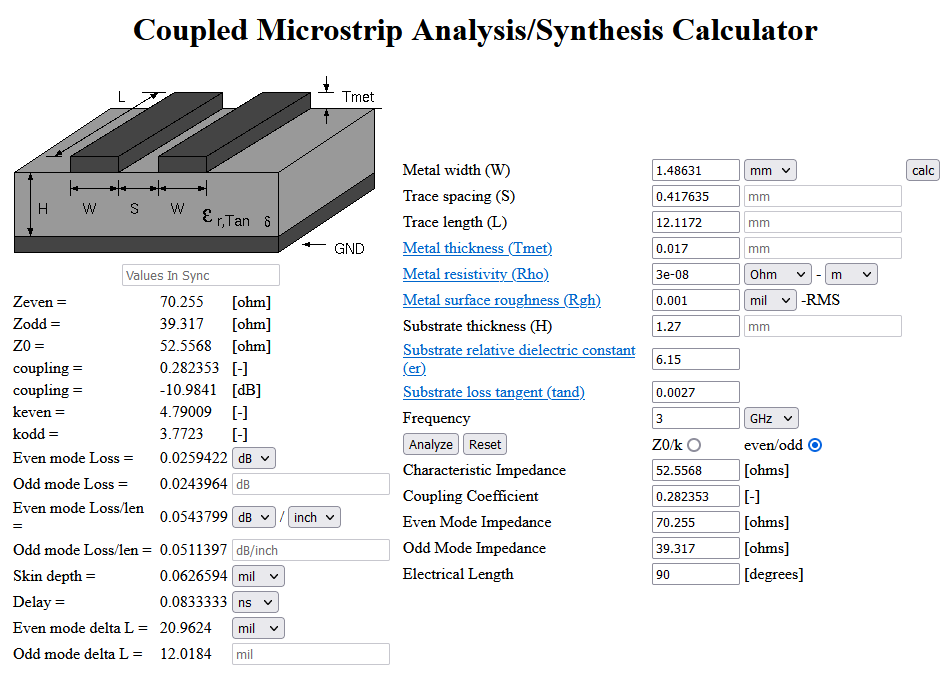
\includegraphics[width=1\linewidth]{images//microstrip_elements/filter_band_pass_microstrip_calculator.png}
    \caption{Calculator of the microstrip coupled lines for the band pass filter}
    \label{fig:microstrip_elements:filter_band_pass_microstrip_calculator}
\end{figure}

If we repeat the process for every coupled line, we get the following results:
\begin{align*}
w_1 &= 1.48631 mm\\
s_1 &= 0.417635 mm \\
l_1 &= 12.1172 mm \\
\\
w_2 &= 1.84182 mm \\
s_2 &= 2.19832 mm \\
l_2 &= 11.8295 mm \\
\\
w_3 &= 1.85223 mm \\
s_3 &= 2.91747 mm \\
l_3 &= 11.8078 mm \\
\\
w_4 &= 1.85315 mm \\
s_4 &= 3.04061 mm \\
l_4 &= 11.8054 mm \\
\\
w_5 &= 1.85223 mm \\
s_5 &= 2.91747 mm \\
l_5 &= 11.8078 mm \\
\\
w_6 &= 1.84178 mm \\
s_6 &= 2.1981 mm \\
l_6 &= 11.8295 mm \\
\\
w_7 &= 1.48631 mm \\
s_7 &= 0.417635 mm \\
l_7 &= 12.1172 mm \\
\end{align*}

Where:
\begin{align*}
    &\text{w: is the width of the coupled line} \\
    &\text{h: is the height of the coupled line} \\
    &\text{s: is the separation of the coupled line} \\
\end{align*}

\subsection{MCLIN implentation}

With all the sections calculates, we can implement the circuit in AWR using MCLIN coupled lines (see Figure \ref{fig:microstrip_elements:fitler_coupled_lines_mclin_circuit}). For the simulation shown in Figure \ref{fig:microstrip_elements:filter_coupled_lines_mclin_graph}, we can see that the band pass filter is working correctly.

\begin{figure}[htbp]
    \centering
    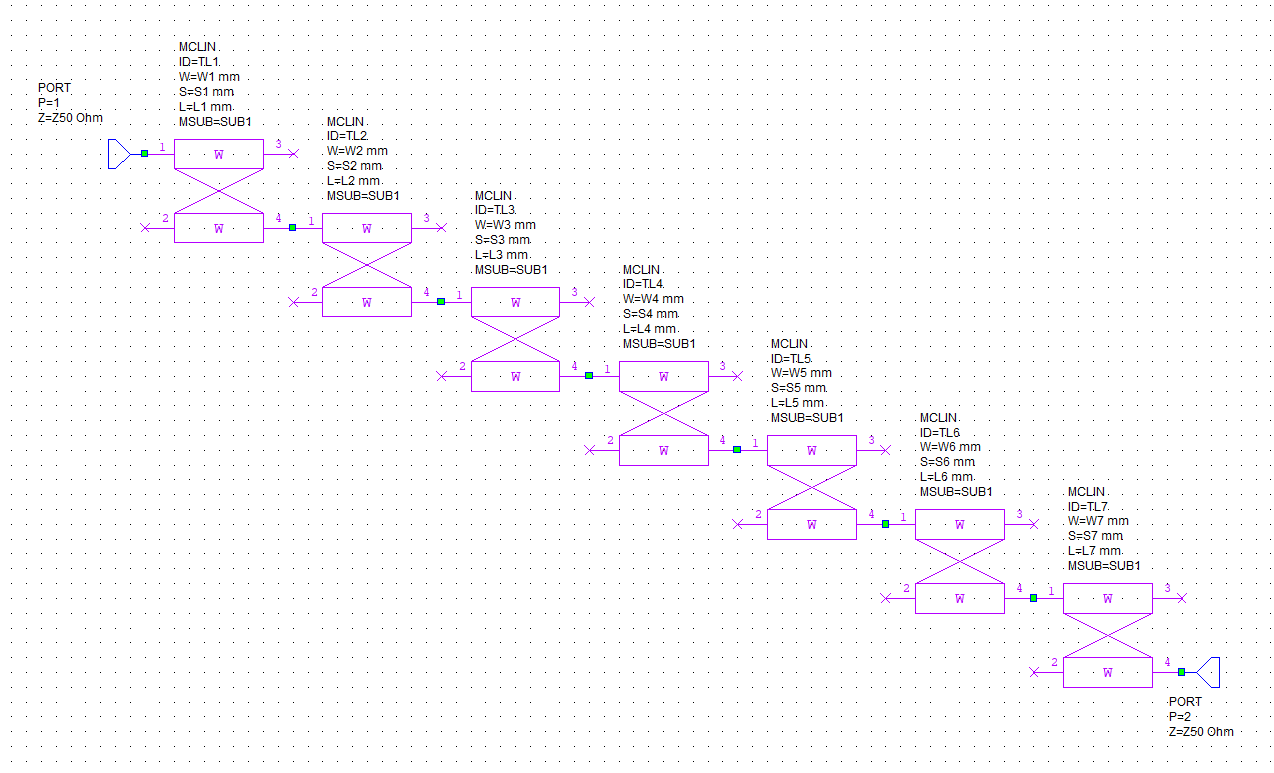
\includegraphics[width=1\linewidth]{images//microstrip_elements/fitler_coupled_lines_mclin_circuit.png}
    \caption{Circuit for the band pass filter implemented with MCLIN coupled lines}
    \label{fig:microstrip_elements:fitler_coupled_lines_mclin_circuit}
\end{figure}

\begin{figure}[htbp]
    \centering
    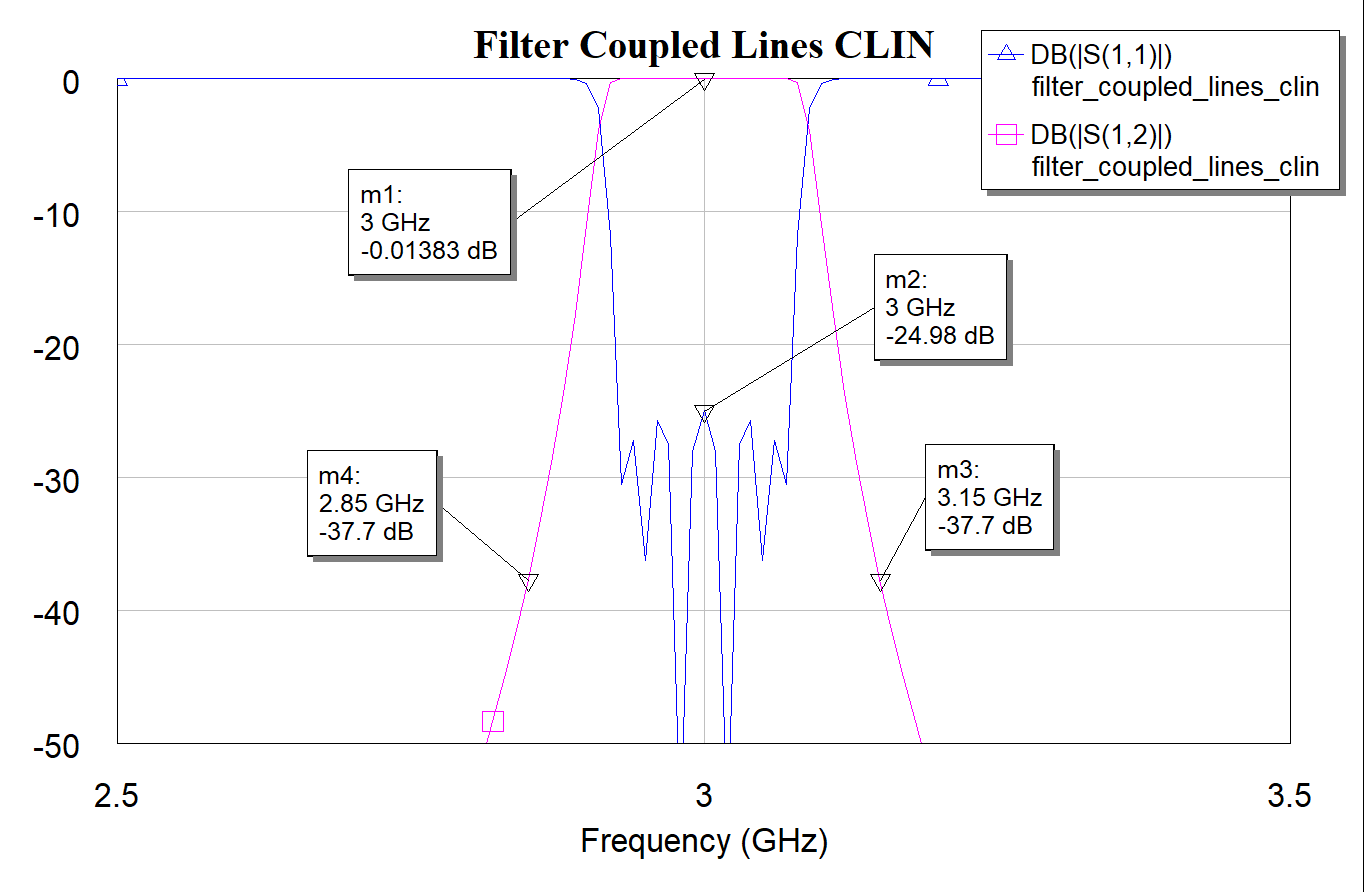
\includegraphics[width=1\linewidth]{images//microstrip_elements/filter_coupled_lines_mclin_graph.png}
    \caption{Simulation of the band pass filter with MCLIN coupled lines (see Figure \ref{fig:microstrip_elements:fitler_coupled_lines_mclin_circuit})}
    \label{fig:microstrip_elements:filter_coupled_lines_mclin_graph}
\end{figure}

\subsection{MCFIL implementation}

Now we will implement it with MCFIL lines. In Figure \ref{fig:microstrip_elements:filter_coupled_lines_mcfil_circuit}, we can see the circuit implemented and in Figure \ref{fig:microstrip_elements:filter_coupled_lines_mcfil_graph}, we can see the simulation. Here we can observe that the center frequency of the filter has been shifted to the left to around $f_0 = 2.9 GHz$. This is because the difference in the widths of the coupled lines make the response of the filter shift. So let's fix it by tuning the widths and lengths of the coupled lines.

\begin{figure}
    \centering
    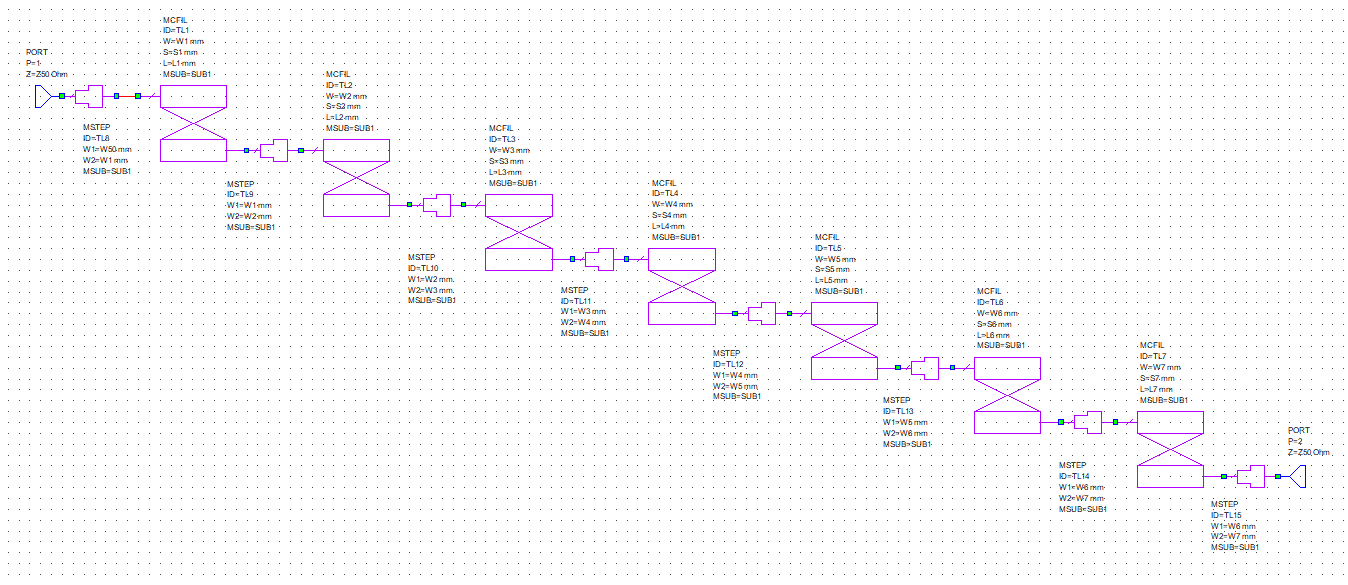
\includegraphics[width=1\linewidth]{images//microstrip_elements/filter_coupled_lines_mcfil_circuit.png}
    \caption{Circuit of the band pass filter with MCFIL coupled lines}
    \label{fig:microstrip_elements:filter_coupled_lines_mcfil_circuit}
\end{figure}

\begin{figure}
    \centering
    \includegraphics[width=1\linewidth]{images//microstrip_elements/filter_coupled_lines_mcfil_graph.png}
    \caption{Simulation of the band pass filter with MCFIL coupled lines (see Figure \ref{fig:microstrip_elements:filter_coupled_lines_mcfil_circuit})}
    \label{fig:microstrip_elements:filter_coupled_lines_mcfil_graph}
\end{figure}

\subsection{MCFIL implementation tuned to our desired characteristics}

After some tuning with the AWR Tune Tool, we got the following dimensions for the different coupled lines for the band pass filter:
\begin{align*}
w_1 &= 1.3 mm\\
s_1 &= 0.417635 mm \\
l_1 &= 11.6 mm \\
\\
w_2 &= 1.4 mm \\
s_2 &= 2.19832 mm \\
l_2 &= 11.5 mm \\
\\
w_3 &= 1.3 mm \\
s_3 &= 2.91747 mm \\
l_3 &= 11.6 mm \\
\\
w_4 &= 1.4 mm \\
s_4 &= 3.04061 mm \\
l_4 &= 11.5 mm \\
\\
w_5 &= 1.3 mm \\
s_5 &= 2.91747 mm \\
l_5 &= 11.6 mm \\
\\
w_6 &= 1.4 mm \\
s_6 &= 2.1981 mm \\
l_6 &= 11.5 mm \\
\\
w_7 &= 1.3 mm \\
s_7 &= 0.417635 mm \\
l_7 &= 11.6 mm \\
\end{align*}

Where:
\begin{align*}
    &\text{w: is the width of the coupled line} \\
    &\text{h: is the height of the coupled line} \\
    &\text{s: is the separation of the coupled line} \\
\end{align*}

For the final circuit, it can be seen in Figure \ref{fig:microstrip_elements:filter_coupled_lines_mcfil_tuned_circuit}. Noticed that we have used MSTEP elements in order to adapt the different widths of the coupled lines. And in the simulation (see Figure \ref{fig:microstrip_elements:filter_coupled_lines_mcfil_tuned_graph}), we can see that now the filter is centered at our desired frequency of $f_0 = 3 GHz$. However, the attenuation at the pass band is a little bit lower than desired, but we where not able to get an attenuation lower than 20 dB.

\begin{figure}[htbp]
    \centering
    \includegraphics[width=1\linewidth]{images//microstrip_elements/filter_coupled_lines_mcfil_tuned_circuit.png}
    \caption{Circuit for the final band pass filter with MCFIL coupled lines}
    \label{fig:microstrip_elements:filter_coupled_lines_mcfil_tuned_circuit}
\end{figure}

\begin{figure}[htbp]
    \centering
    \includegraphics[width=1\linewidth]{images//microstrip_elements/filter_coupled_lines_mcfil_tuned_graph.png}
    \caption{Simulation for the final band pass filter of Figure \ref{fig:microstrip_elements:filter_coupled_lines_mcfil_tuned_circuit}}
    \label{fig:microstrip_elements:filter_coupled_lines_mcfil_tuned_graph}
\end{figure}

\subsection{Layout}

For the layout of the band pass filter, it can be seen in Figure .

\begin{figure}[htbp]
    \centering
    \includegraphics[width=1\linewidth]{images//microstrip_elements/filter_coupled_lines_mcfil_tuned_layout.png}
    \caption{Layout of the final band pass filter of Figure \ref{fig:microstrip_elements:filter_coupled_lines_mcfil_tuned_circuit}}
    \label{fig:microstrip_elements:filter_coupled_lines_mcfil_tuned_layout}
\end{figure}

\section{Directional Coupler}

For the directional coupler, in order to adapt the ideal directional coupler of Figure \ref{fig:design_circuit_elements:directional_coupler_ideal_circuit}, we need to calculate the parameters of the microstrip line.

\subsection{Calculation of the length, width, and separation of the coupled microstrip lines}

In order to calculate the, we used the Tunner Tool of AWR where we modified the length (L), width (W), and separation (S) until we got a coupling of $C = 20 \ dB$ and a reflected power of as low as possible. For this simulation we have used the circuit pictured in Figure \ref{fig:microstrip_elements:directional_coupler_real_circuit}. Notice that the elements on the coupled port are just to be able to be implemented in the microstrip technology to have space in the PCB to place the elements. 

\begin{figure}[htbp]
    \centering
    \includegraphics[width=1\linewidth]{images//microstrip_elements/directional_coupler_real_circuit.png}
    \caption{Circuit of the final directional coupler implementation}
    \label{fig:microstrip_elements:directional_coupler_real_circuit}
\end{figure}

The simulation can be seen in the Figure \ref{fig:microstrip_elements:directional_coupler_real_graph}. Here we can observer that the microstrip implementation is as good as the ideal implementation (see Figure \ref{fig:design_circuit_elements:directional_coupler_ideal_graph}).

\begin{figure}
    \centering
    \includegraphics[width=1\linewidth]{images//microstrip_elements/directional_coupler_real_graph.png}
    \caption{Simulation of the directional coupler shown in Figure \ref{fig:microstrip_elements:directional_coupler_real_circuit}}
    \label{fig:microstrip_elements:directional_coupler_real_graph}
\end{figure}

\subsection{Layout}

For the layout, it can be seen in Figure \ref{fig:microstrip_elements:directional_coupler_real_layout}.

\begin{figure}[htbp]
    \centering
    \includegraphics[width=1\linewidth]{images//microstrip_elements/directional_coupler_real_layout.png}
    \caption{Layout of the directional coupler shown in Figure \ref{fig:microstrip_elements:directional_coupler_real_circuit}}
    \label{fig:microstrip_elements:directional_coupler_real_layout}
\end{figure}

%-------------------------------------
\chapter{Integration}

\section{Common Microstrip Layout}

The full circuit implementation can be seen in Figure \ref{fig:integration:complete_circuit_circuit} and the layout can be seen in Figure \ref{fig:integration:complete_circuit_layout}. One thing to take into consideration is that we have added TLs at the end of the ports in order to give some room in the PCB to solder the elements. And also, we did not need to add any matching elements as the circuits where matched to a characteristic impedance of $Z_0 = 50 \Omega$, thus not needing any further matching.

\begin{figure}[htbp]
    \centering
    \includegraphics[width=1\linewidth]{images//integration/complete_circuit_circuit.png}
    \caption{Full circuit schematics}
    \label{fig:integration:complete_circuit_circuit}
\end{figure}

\begin{figure}[htbp]
    \centering
    \includegraphics[width=1\linewidth]{images//integration/complete_circuit_layout.png}
    \caption{Layout of the complete circuit of Figure \ref{fig:integration:complete_circuit_circuit}}
    \label{fig:integration:complete_circuit_layout}
\end{figure}

\section{Simulation of the Full Network at Working Frequencies}

In the Figure \ref{fig:integration:complete_circuit_graph_working_freq}, we can observe the response of our circuit at the working frequencies. Here we can observe that the 2 stage amplifier works at the desired pass band with a gain of $G = 28.71 dB$ and an attenuation almost negligible. On the other hand, at the other frequencies, the filter does not allow any frequency through.

\begin{figure}[htbp]
    \centering
    \includegraphics[width=1\linewidth]{images//integration/complete_circuit_graph_working_freq.png}
    \caption{Simulation of the full circuit of Figure \ref{fig:integration:complete_circuit_circuit} at working frequencies.}
    \label{fig:integration:complete_circuit_graph_working_freq}
\end{figure}

\section{Simulation of the Full Network Wide band Response (0GHz up to 7GHz)}

For the full response of our circuit, it can be seen in Figure \ref{fig:integration:complete_circuit_graph_full_freq}. Here we can see that the circuit works at expected as it only allows the desired frequency. However, at $f = 6 GHz$, the filter allows the signal to be amplified. This is because the filter we have implemented has resonant frequencies and this is one of them.

\begin{figure}[htbp]
    \centering
    \includegraphics[width=1\linewidth]{images//integration/complete_circuit_graph_full_freq.png}
    \caption{Simulation of the full circuit of Figure \ref{fig:integration:complete_circuit_circuit} at the full range of frequencies}
    \label{fig:integration:complete_circuit_graph_full_freq}
\end{figure}

%-------------------------------------
\chapter{Results and Conclusions}

\section{Comparison of the System Specifications with the Simulated Results}

For the final results we will comparing the simulated results to the requirements for the circuit. We will use the simulation in Figure \ref{fig:results:graph} to make the comparisons.

\begin{figure}[htbp]
    \centering
    \includegraphics[width=1\linewidth]{images//results/graph.png}
    \caption{Simulation of the final circuit with interesting markers}
    \label{fig:results:graph}
\end{figure}

\begin{itemize}
    \item  We can see that the centered frequency $f_0 = 3 GHz$ is the same as the requirements. 
    \item For the bandwidth, in the simulation we can see that it goes from $2.925 GHz$ to $3.075 GHz$; which is the same as the specifications stated.
    \item For the gain of the amplifier, we get the same results calculated previously of $28 dB$.
    \item The return loss at the input port of our circuit is $15 dB$ which does not pass the requirements of $30 dB$. However, after trying to tune the filter and coupled lines we were not able to achieve any higher return loss at the input port.
    \item For the return loss at the output port, we get $16 dB$ which is close to the requirement of $18 dB$. We were able to increase the return loss by tuning the circuit but not to get the required return loss.
    \item For the attenuation outside the pass band, we get an attenuation much lower than 25 dB that were required.
    \item Finally, for the power at the monitor, we get exactly 20 dB lower to the main output port.
\end{itemize}

\section{Conclusions} 

The design and characterization of a two-stage, balanced microwave amplifier represent a significant achievement in the field of high-frequency technologies. Through theoretical analysis and practical implementation, we have successfully met the objectives outlined in this laboratory exercise. Our design approach was guided by the need to overcome inherent limitations of amplifiers, focusing on maximizing gain while ensuring efficient power utilization.

The first stage of our amplifier utilized a commercial integrated amplifier, GVA-83+, configured as a simple amplifier. By leveraging data provided by the manufacturer and implementing bias and DC block networks, we ensured proper operation within specified parameters. Additionally, the balanced second stage, featuring phase shifters and Wilkinson power dividers/combiners, enabled enhanced performance and power distribution. Through careful design and simulation, we achieved the desired specifications, including a center frequency within the desired range, high gain, and effective suppression of out-of-band frequencies.

Furthermore, our design process involved the meticulous design and integration of other crucial components such as the band pass filter and directional coupler. These elements, designed with microstrip technology, contributed to the overall functionality and performance of the amplifier. Our comprehensive approach, from theoretical analysis to practical implementation and simulation, has resulted in a robust and efficient microwave amplifier design. However, further optimization and refinement may be warranted to address any discrepancies between simulated and desired specifications, ensuring the amplifier meets the highest standards of performance and reliability in real-world applications.

%----------
%	BIBLIOGRAFÍA
%----------	

%\nocite{*} % Si quieres que aparezcan en la bibliografía todos los documentos que la componen (también los que no estén citados en el texto) descomenta está línea

\clearpage
\addcontentsline{toc}{chapter}{Bibliografía}
%\setquotestyle[english]{british} % Cambiamos el tipo de cita porque en el estilo IEEE se usan las comillas inglesas.
\printbibliography


%----------
%	ANEXOS
%----------	

% Si tu trabajo incluye anexos, puedes descomentar las siguientes líneas
%\chapter* {Anexo x}
%\pagenumbering{gobble} % Las páginas de los anexos no se numeran



\end{document}